% -*-memoria.tex-*-
% Este fichero es parte de la plantilla LaTeX para
% la realización de Proyectos Final de Carrera, protegido
% bajo los términos de la licencia GFDL.
% Para más información, la licencia completa viene incluida en el
% fichero fdl-1.3.tex

% Copyright (C) 2009 Pablo Recio Quijano 

%-------------------------------------------------------
% ---- Plantilla para libros / memorias PFC -----

% Realizada por Pablo Recio Quijano y Noelia Sales Montes 
% Formato de portada y primera página tomado del PFC de
% Francisco Javier Vázquez Púa, en su proyecto 'libgann'
% -------------------------------------------------------

\documentclass[a4paper,11pt]{book}

\usepackage{./estilos/estiloBase} % Basicamente son todas las
                                  % librerias usadas. En caso de que
                                  % falten librerias se van añadiendo
                                  % al fichero.
\usepackage{./estilos/colores}  % Algunos colores ya generados, para
                                % los algunos estilos más avanzados.
\usepackage{./estilos/comandos} % Algunos comandos personalizados

\graphicspath{{./imagenes/}} % Indicamos la ruta donde se encuentran
                             % las imagenes, para ahorrarnos la ruta
                             % completa, y solo modificar aquí si en
                             % un momento dado lo movemos

\begin{document}

% Renombramos las figuras y las tablas
\renewcommand{\figurename}{Figura}
\renewcommand{\listfigurename}{Indice de figuras}
\renewcommand{\tablename}{Tabla}
\renewcommand{\listtablename}{Indice de tablas}

\pagestyle{empty}
% -*-portada.tex-*-
% Este fichero es parte de la plantilla LaTeX para
% la realización de Proyectos Final de Carrera, protejido
% bajo los términos de la licencia GFDL.
% Para más información, la licencia completa viene incluida en el
% fichero fdl-1.3.tex

% Fuente tomada del PFC 'libgann' de Javier Vázquez Púa

\begin{titlepage}

  \begin{center}

    
\includegraphics[scale=0.2]{logo_uca.png} \\
    
    \vspace{2.0cm}
    
    \LARGE{\textbf{ESCUELA SUPERIOR DE INGENIERÍA}} \\
    
    \vspace{1.0cm}
    
    \Large{\textbf{Evaluación de competencias mediante la extracción de indicadores procedentes de los registros de actividad de los entornos de aprendizaje virtuales. Un Estudio de Mapeo Sistemático}} \\
    
    \vspace{3.0cm}
    
    \Large{Trabajo de Investigación} \\
    
    \vspace{2.0cm}
    
    \Large{Antonio Balderas Alberico} \\
  
    \vspace{0.5cm}

    \large{\today}
    
  \end{center}
\end{titlepage}

\cleardoublepage

% -*-primerahoja.tex-*-
% Este fichero es parte de la plantilla LaTeX para
% la realización de Proyectos Final de Carrera, protejido
% bajo los términos de la licencia GFDL.
% Para más información, la licencia completa viene incluida en el
% fichero fdl-1.3.tex

% Fuente tomada del PFC 'libgann' de Javier Vázquez Púa

\begin{center}

  
\includegraphics[scale=0.2]{logo_uca.png} \\

  \vspace{2.0cm}

  \Large{ESCUELA SUPERIOR DE INGENIERÍA} \\

  \vspace{1.0cm}

  \large{Itinerario Formativo de Doctorado 7009} \\

  \vspace{2.0cm}

  \large{Trabajo de Investigación} \\

  \vspace{1.0cm}

  \Large{\textbf{Evaluación de competencias mediante la extracción de indicadores procedentes de los registros de actividad de los entornos de aprendizaje virtuales}} \\
    
  \vspace{3.0cm}

\end{center}

\begin{itemize}
\item \large{Departamento: Ingeniería Informática}
\item \large{Autor: Antonio Balderas Alberico}
\item \large{Tutores: Manuel Palomo Duarte y Juan Manuel Dodero Beardo}
\end{itemize}

\vspace{1.0cm}

\begin{flushright}
  \large{Cádiz, \today} \\

\end{flushright}

\cleardoublepage
\pagestyle{plain}

\frontmatter % Introducción, índices ...

%% -*-previo.tex-*-
% Este fichero es parte de la plantilla LaTeX para
% la realización de Proyectos Final de Carrera, protejido
% bajo los términos de la licencia GFDL.
% Para más información, la licencia completa viene incluida en el
% fichero fdl-1.3.tex

% Copyright (C) 2009 Pablo Recio Quijano 

\section*{Agradecimientos}

Me gustaria agradecer y/o dedicar este texto a Rafael Gordillo y Robert Jarni.

\cleardoublepage

\section*{Licencia} % Por ejemplo GFDL, aunque puede ser cualquiera

Este documento ha sido liberado bajo Licencia GFDL 1.3 (GNU Free
Documentation License). Se incluyen los términos de la licencia en
inglés al final del mismo.\\

Copyright (c) 2009 Pablo Recio Quijano.\\

Permission is granted to copy, distribute and/or modify this document under the
terms of the GNU Free Documentation License, Version 1.3 or any later version
published by the Free Software Foundation; with no Invariant Sections, no
Front-Cover Texts, and no Back-Cover Texts. A copy of the license is included in
the section entitled "GNU Free Documentation License".\\

\cleardoublepage

\section*{Notación y formato}

Aquí incluiremos los aspectos relevantes a la notación y el formato a
lo largo del documento. Para simplificar podemos generar comandos
nuevos que nos ayuden a ello, ver \texttt{comandos.sty} para más
información. 

Cuando nos refiramos a un programa en concreto, utilizaremos la
notación: \\ \programa{emacs}.\\

Cuando nos refiramos a un comando, o función de un lenguaje, usaremos
la notación: \\ \comando{quicksort}.\\
\cleardoublepage

\tableofcontents
\listoffigures
\listoftables

\mainmatter % Contenido en si ...

\chapter{Introducción}
% INTRODUCCION

En los últimos años, el interés en la evaluación del aprendizaje ha cambiado del conocimiento a las competencias. Proyectos como el \emph{Tuning Educational Structures in Europe}, apoyado por el Lifelong Learning Program de la Unión Europea, muestran la importancia de utilizar el concepto de competencia como base para los resultados de aprendizaje. Las competencias de aprendizaje son habilidades que un alumno ha de ser capaz de demostrar una vez que termina su formación. Estas competencias de aprendizaje se dividen en dos grupos: específicas y genéricas. Competencias específicas son aquellas relacionadas directamente con la utilización de conceptos, teorías o habilidades propias de un área en concreto, mientras que las competencias genéricas son habilidades, capacidades y conocimientos que cualquier estudiante debería desarrollar independientemente de su área de estudio \cite{Tuning:2003}. Aunque obviamente sigue siendo muy importante el desarrollo del conocimiento específico de cada área de estudio, es un hecho que el tiempo y la atención también deben dedicarse al desarrollo de las competencias genéricas. Igualmente es importante reconocer la aplicación de dichas habilidades genéricas fuera del ámbito académico, ya que son cada vez más relevantes para la preparación de estudiantes para su futuro papel en la sociedad, en términos de empleabilidad y ciudadanía.

Sin embargo, evaluar ciertas competencias genéricas es a menudo una tarea bastante subjetiva, lo que es problemático tanto para el profesor como para los alumnos. A menos que una competencia genérica está directamente enlazada a una actividad específica, éstas son difíciles de evaluar. Desarrollar un procedimiento detallado para la evaluación en el desempeño de los estudiantes en las competencias genéricas es una actividad compleja y que requiere mucho tiempo por los diferentes aspectos a tener en cuenta. Si el profesor apenas tiene tiempo suficiente durante el curso académico para cumplir su planificación y evaluar todas las tareas, exámenes o trabajos que los alumnos han tenido que realizar para demostrar la adquisición de competencias específicas en una asignatura, difícilmente podrá asumir la carga adicional que supone una evaluación detallada, objetiva y justificada de determinadas competencias genéricas. Por lo que, aunque un alumno haya superado una asignatura, no siempre se podría garantizar que éste sea capaz de desempeñar las competencias genéricas recogidas en su plan de estudios.

Debido a la rápida transformación de una sociedad que se basa en el conocimiento y a los sistemas de educación, vivimos en un contexto donde las habilidades demandadas son cambiantes. Cada vez es más evidente que los planes de estudio, y con ellos las estrategias de evaluación, deben centrarse en un enfoque más integral de las competencias genéricas y específicas. Las TIC ofrecen muchas oportunidades para el apoyo a los formatos de evaluación que pueden capturar habilidades complejas y competencias que son difíciles de evaluar \cite{Redecker:2013}. Si los planes de estudio y los objetivos de aprendizaje han cambiado, también deberían hacerlo las prácticas de evaluación \cite{Cachia:2011}.

El ámbito de nuestro trabajo está relacionado con los entornos de aprendizaje virtual: LMS y VLE (LMS, Learning Management System y VLE, Virtual Learning Environment). Los entornos LMS o VLE pueden ser tanto entornos monolíticos y holísticos donde se desarrollan y gestionan experiencias virtuales, como ser un entorno basado en las tecnologías semánticas y \emph{linked data}, y estar constituidos por una miríada de herramientas, plataformas y servicios independientes \cite{Dodero:2013}. Estos entornos están diseñados especialmente para incluir no sólo tareas individuales, sino también tareas colaborativas como foros o wikis. \emph{Un foro es una aplicación web que da soporte a discusiones u opiniones en línea} (Wikipedia), mientras que \emph{un wiki es un tipo de página web que brinda la posibilidad de que multitud de usuarios puedan editar sus contenidos a través del navegador web, con ciertas restricciones mínimas} (Wikipedia). Todos ellos son muy empleados como soporte para clases presenciales, haciendo más fácil la comunicación con los estudiantes y manteniendo siempre disponibles las actividades y recursos para el tema \cite{Zafra:2011, Munkhchimeg:2013}. Además, son ampliamente utilizados hoy en día por los centros educativos a todos los niveles, facilitando la descontextualización y fomentando en muchos casos una motivación extra del estudiante mediante un juego (GBL) con un posible componente competitivo \cite{Bellotti:2013,Berns:2013,Palomo-Duarte:2012}.

Cuando el número de alumnos es elevado, se hace mucho menos escalable la evaluación para el profesor. Por ejemplo, este tipo de situaciones se suele dar en los MOOC (Massive Open Online Course), cuya filosofía es la liberación del conocimiento, para que este llegue a un público más amplio, y para el que se suelen ofrecer plazas ilimitadas \cite{Lugton:2012, Mor:2013}. Este tipo de curso, que también se caracteriza por ser de carácter abierto y gratuito, y con materiales accesibles de forma gratuita, presenta evidentes problemas de escalabilidad cuando la evaluación no está automatizada \cite{Johnson:2013}.

En los LMS, cada archivo subido, cada actividad realizada, cada acceso al sistema o cada comentario escrito en un foro por los estudiantes queda registrado en el sistema. Según \cite{Chebil:2012, Florian:2011} la recopilación de los rastros de interacción producidos por estos entornos TEL (Technology Enhanced Learning), aunque con su correspondiente filtrado, puede ser una información muy valiosa para obtener indicadores del desempeño de los alumnos en competencias genéricas.

El objetivo de este trabajo de investigación es realizar un análisis de la literatura para conocer hasta qué punto la ciencia informática se ha ocupado de la evaluación de competencias genéricas, prestando especial atención en aquellos trabajos que realicen dicha evaluación de manera automatizada aprovechando las prestaciones de las nuevas tecnologías. Consideramos que la información almacenada en la base de datos de un LMS puede ser aprovechada para extraer indicadores que proporcionen una medida objetiva del desempeño de los alumnos en ciertas competencias genéricas. ¿Cuántos trabajos han tratado esta problemática anteriormente? ¿Qué competencias pueden ser evaluadas de manera automática? Todas estas dudas, serán planteadas de manera formal en en el siguiente capítulo, dónde se darán las indicaciones de la metodología seguida. A continuación se mostrarán los resultados, las respuestas a las preguntas, el trabajo futuro y por último las conclusiones y la bibliografía utilizada.






\chapter{Metodología}
% -*-cap2_metodologia.tex-*-

Un Estudio de Mapeo Sistemático (SMS, Systematic Mapping Study), es una amplia revisión de los estudios primarios en un area específica cuyo objetivo es identificar alguna evidencia sobre el tema. Este estudio se basa en las directrices publicadas en la metodología propuesta por Kitchenham \cite{Kitchenham:2010}. Esta metodología describe cómo se deben planificar, ejecutar y presentar los resultados de una revisión de la literatura en la ingeniería del software. Para este trabajo se ha utilizado la propuesta de Petersen \cite{Petersen:2008}.

Es muy importante seguir un procedimiento sistemático para llevar a cabo una revisión rigurosa de la literatura. En un primer momento, se trató de seguir la clasificación aportada por \cite{Redecker:2012} para el ámbito de aplicación de la contribución. En él se plantea una división generacional:
\begin{itemize}
\item Primera generación: administración y calificación automatizada de pruebas convencionales
\item Segunda generación: pruebas adaptativas
\item Tercera generación: evaluación integrada continua
\item Cuarta generación: retroalimentación tutorizada y personalizada
\end{itemize}
Sin embargo, la selección de la literatura realizada en este trabajo, no se adaptaba a esta categorización, por lo que finalmente los artículos fueron agrupados según el tipo de herramienta, modelo, paradigma o discusión que planteaban. La clasificación final fue:
\begin{itemize}
\item Course’s Learning Outcomes (CLO) and rubrics: trabajos que evalúan las competencias genéricas de los alumnos a partir de rúbricas de los resultados del trabajo de los alumnos
\item Peer and self eAssessment: trabajos que delegan la función de evaluar competencias genéricas en los compañeros o en la autoevaluación
\item Game-Based Learning (GBL): trabajos que se basan en juegos para la evaluación de competencias genéricas
\item eAssessment and reviews: resto de trabajos que agrupan propuestas para la evaluación de competencias genéricas mediante el uso de la tecnología 
\end{itemize}

\section{Justificación}
El motivo de este trabajo, tal como se describió en la introducción, es la localización de trabajos relacionados con la tecnología para la mejora del aprendizaje (TEL) cuyo fin sea la evaluación de competencias de manera automática. El contexto de esta investigación viene marcado por la problemática del ``Open Data``. En la era de la Web 2.0, dispositivos como los gadgets de iGoogle se están convirtiendo cada vez más populares para la integración y personalización de contenidos Web de diferentes fuentes. Estas nuevas tecnologías de la Web se pueden aprovechar como portales de ciencia en términos de interfaz de usuario dinámica, que impulse la implementación de pasarelas con fines de educación avanzada, y así convirtiendo los datos en accesibles y reutilizables \cite{Wenjun:2008}.

Los entornos de aprendizaje virtual (LMS ó VLE) almacenan información de estudiantes, profesores, cursos, tareas, trabajos, etc. Estos elementos se relacionan y configuran para ofrecer al usuario una experiencia de curso virtual. Haciendo todos estos datos almacenados accesibles, siguiendo la filosofía de ``Open Data``, se podría sacar partido a los mismos con fines científicos. Y tal como se comentó en la introducción, para que esta evaluación de competencias sea escalable y más aún cuando el número de alumnos es importante, no queda otra alternativa que hacerlo de manera automatizada.

% Añadir despues de con fines científicos \cite{PENDIENTE:CITA:REGISTROS:ALMACENADOS:LMS}

\section{Preguntas de investigación}

En este punto, hemos de plantearnos cuáles son las cuestiones que necesitamos resolver para llevar a cabo nuestra investigación. Necesitamos saber en qué punto se haya la comunidad científica en lo que se refieres al uso de los registros de los entornos de aprendizaje para evaluar las competencias genéricas. Para ello planteamos la primera pregunta: \emph{¿Cuáles son las competencias que se han evaluado de forma automática o asistida por ordenador a partir del uso de los entornos virtuales?}

Además, necesitamos saber de qué forma lo hace, qué métodos y técnicas se utilizan para este fin. Para eso se plantean las preguntas segunda (\emph{¿Qué herramientas o metodologías se utilizan para evaluar competencias mediante el uso de los entornos virtuales?})y tercera (\emph{¿Con qué técnicas se pueden obtener evidencias (numéricas) objetivas del desarrollo de las siguientes competencias en un entorno virtual?}).

Finalmente se necesita saber si los resultados que se obtengan de los registros de interacción de un sistema LMS realmente reflejan el desempeño o no de los estudiantes en qué competencia, planteádose por tanto la cuarta pregunta: \emph{¿Los resultados que se obtendrían de la evaluación de competencias genéricas de los alumnos mediante el uso de los registros de actividad de los entornos virtuales son indicadores fiables del desempeño de dichas competencias?}.

\bigskip
Preguntas de investigación:
\begin{enumerate}
%\item ¿Cuáles son las competencias que se han evaluado de forma automática o asistida por ordenador a partir del uso de los LMS?
%\item ¿Qué métodos y técnicas se utilizan para evaluar competencias mediante el uso de un LMS?
%\item ¿Con qué técnicas se pueden obtener evidencias (numéricas) objetivas del desarrollo de las siguientes competencias en un LMS?
%\item ¿Los resultados que se obtendrían de la evaluación de competencias genéricas de los alumnos mediante el uso de los registros de actividad de los LMS son indicadores fiables del desempeño de dichas competencias?
\item ¿Cuáles son las competencias que se han evaluado de forma automática o asistida por ordenador a partir del uso de los entornos virtuales?
\item ¿Qué herramientas o metodologías se utilizan para evaluar competencias mediante el uso de los entornos virtuales?
\item ¿Con qué técnicas se pueden obtener evidencias (numéricas) objetivas del desarrollo de las siguientes competencias en un entorno virtual?).
\item ¿Los resultados que se obtendrían de la evaluación de competencias genéricas de los alumnos mediante el uso de los registros de actividad de los entornos virtuales son indicadores fiables del desempeño de dichas competencias?
\end{enumerate}

\section{Protocolo de revisión}

La definición del protocolo de revisión requiere la realización de una serie de acciones para obtener la bibliografía de nuestro estudio. Comenzaremos indicando los motores de búsqueda que vamos a utilizar, qué términos de búsqueda utilizaremos en dichos motores y las herramientas de soporte a la revisión. Además se mostrarán qué criterios de inclusión de la bibliografía se siguen y el procedimiento de selección.
% Incluir algo de 'Esquema para la extracción de datos'??

\subsection{Motores de búsqueda}
Una vez que las preguntas de la investigación se han establecido, hay que identificar con precisión la estrategia de búsqueda a seguir. En nuestro procedimiento, para encontrar la bibliografía, se realizarán consultas en las siguientes bibliotecas digitales: Wiley Online Library, World Scientific Net, Springer, ACM Digital Library, IEEE Digital Library (Xplore) y Scopus.

\subsection{Términos de búsqueda}
\label{sec:TerminosBusqueda}
Existen muchos términos que pueden utilizarse para referirse a la evaluación de competencias genéricas de manera automatizada o asistida. Por la naturaleza de nuestro trabajo, debemos contemplar siempre en las palabras de búsqueda los términos ``assessment`` y ``generic skills`` o ``generic competences``. Realizar la búsqueda por el término ``Assessment of generic skills`` o ``assessing generic skills`` nos planteaba la primera problemática, y es que el número de artículos devueltos era muy reducido. Sin embargo, debilitar la búsqueda con términos como ``generic competences`` o ``generic skills`` junto con la palabra ``assessment`` daba un número de resultados muy elevado. En primera instancia se probó añadiendo términos como  ``E-Learning``, ``computer-assisted`` o ``mobile learning``. Sin embargo, incluir términos de este tipo reducían también drásticamente el número de resultados obtenidos en la búsqueda, no llegando a obtenerse bibliografía más significativa que si no se incluyen. Por tanto, a tenor de las pruebas se decide eliminar de la búsqueda ese tipo de términos. Por otro lado, sí se incluyen acrónimos de diferentes entornos virtuales relacionados con las TEL, como son: ``TEL``, ``LMS``, ``ICT`` (Information and communications technology) , ``CBI`` (Content-Based Instruction). Y tras varias pruebas, se descartan también de la búsqueda términos como ``ICE`` (Integrated Collaboration Environment) y ``CSCL`` (Computer Supported Collaborative Learning). La combinación de los términos de búsqueda empleados en la investigación, así como a los motores de búsqueda que fueron aplicados en cada una pueden comprobarse en la tabla \ref{tab:ResumenBusqueda}.

\begin{table}[H]
  \begin{center}
  \begin{tabular}{| m{4cm} | m{7cm} | m{3cm} |}
    \hline
    SOURCE & SEARCH TERMS & SEARCH SCOPE \\
    \hline
    \hline
    Wiley Online Library & assessment AND ``generic competences`` OR ``generic skills`` AND (TEL OR ICT OR CBI) & in All Fields\\
    \hline
    World Scientific Net & ``generic competences`` OR ``generic skills`` AND assessment & Anywhere in article\\
    \hline
    Springer & (``generic skills`` OR ``generic competences``) AND  students AND (TEL OR CBI OR ICT) & All fields (Including full text)\\
    \hline
    ACM Digital Library & (assessment and ``generic skills``) and (TEL or LMS or ICT or CBI) & Any field (title, abstract, review)\\
    \hline
    ACM Digital Library & (assessment and ``generic competences``) and (TEL or LMS or ICT or CBI) & Any field (title, abstract, review)\\
    \hline
    IEEE Digital Library (Xplore) & (((TEL or LMS or ICT or CBI) AND (``generic skills`` OR ``generic competences``)) AND assessment) & Full text and metadata\\
    \hline
    Scopus & (((TEL or LMS or ICT or CBI) AND (``generic skills`` OR ``generic competences``)) AND assessment) & All fields (Including full text)\\
    \hline
  \end{tabular}
\end{center}
\caption{Resumen de búsqueda de bibliografía}
\label{tab:ResumenBusqueda}
\end{table} 

% Incluir tabla con resultados descartados (Supongo que en anexo).

\subsection{Criterios de selección}
Para determinar si un trabajo debía formar parte de nuestra selección de estudios primarios se leyó tanto el título, como el resumen y las palabras clave. En ocasiones, esto no es suficiente, siendo necesario complementar la lectura anterior con una somera la lectura del artículo completo y más detallada de la introducción y las conclusiones.
Nuestra búsqueda se centra en la localización de los trabajos que, habiendo sido obtenidos en el proceso de búsqueda anterior, vayan en línea con nuestro estudio y puedan ayudarnos a resolver las preguntas de investigación. Para ello, se realizó la proyección de los trabajos seleccionados utilizando los siguientes criterios de exclusión:
\begin{itemize}
\item Off Topic: trabajo no relacionado directamente con nuestra investigación. Son trabajos, que aún satisfaciendo los criterios de búsqueda porque de alguna forma se mencionan en el texto, después su contribución no está relacionada con la evaluación asistida de competencias genéricas.
\item Unsupported Language: Trabajo escrito en un lenguaje diferente al inglés o español. La mayoría de los textos son en inglés, por lo que este criterio de descarte apenas es utilizado.
\item Duplicated: Trabajos cuya contribución principal está recogida en otros trabajos ya incluidos. 
\item Unread: Trabajo que no ha podido ser leido. Son textos que no han sido leídos al no estar disponible para su lectura en las bibliotecas digitales a las que tenemos acceso desde la Universidad. Así mismo, aunque algún artículo ha podido ser encontrado gracias a Google Scholar o a la generosidad de sus autores, alguno ha quedado pendiente de lectura.
\end{itemize}

%Para considerar que un trabajo está relacionado directamente con nuestra contribución ha de ayudarnos a resolver alguna de las preguntas de investigación. Por tanto, un trabajo se incluye si:
%\begin{itemize}
%\item Realizan una evaluación automática de competencias genéricas
%\item Realizan una evaluación de competencias genéricas apoyándose en la tecnología, aunque no de manera automática
%\item Realizan una evaluación de alguna competencia específica apoyándose en la tecnología, utilizando alguna técnica cuya aplicación poduera ser de interés para nuestro estudio
%\item Trabajos que abordan la evaluación de competencias genéricas
%\end{itemize}

\subsection{Esquema para la extracción de datos}

Para la extracción de la información dividiremos los trabajos según el tipo de investigación que realizan.

\subsubsection{Tipo de investigación}
Esta clasificación hace referencia al tipo de trabajo de investigación llevado a cabo por el/los investigador/es. Según los autores existen diferentes enfoques para la investigación. Algunos de estos sistemas de clasificación son los propuestos por Wieringa \cite{Wieringa:2005} y Hevner \cite{Hevner:2004}. Usamos el primero, ya que es el recomendado en el proceso de mapeo sistemático descrito por Petersen \cite{Petersen:2008}.
\begin{itemize}
\item Solución propuesta (\emph{proposal of solution}): se propone una solución para un problema; la solución puede ser innovadora o una extensión significativa de una técnica existente. Los posibles beneficios y la aplicabilidad de la solución se demuestran por un pequeño ejemplo o una buena línea de argumentación.
\item Validación de investigación (\emph{validation research}): las técnicas investigadas son nuevas y todavía no se han aplicado en la práctica. Estas técnicas podrían ser por ejemplo los experimentos, es decir, el trabajo realizado en un laboratorio.
\item Evaluación de la Investigación (\emph{evaluation research}): las técnicas se aplican en la práctica y se lleva a cabo una evaluación de la técnica. Se muestra cómo se implementa la técnica en la práctica (implementación de la solución) y cuáles son las consecuencias de la aplicación en términos de ventajas y desventajas (evaluación de implementación).
\item Artículos de Experiencia (\emph{experience papers}): trabajos que explican qué y cómo algo se ha llevado a cabo en la práctica. Basado en la experiencia personal del autor.
\item Artículos de opinión (\emph{opinion papers}): estos trabajos expresan la opinión personal de alguien acerca de si una determinada técnica es buena o mala, o cómo se deben realizar las cosas. No se basan en metodologías de trabajo y de investigación relacionadas.
\item Trabajos filosóficos (\emph{philosophical papers}): estos trabajos esbozan una nueva forma de ver las cosas existentes, estructurando el campo en forma de una taxonomía o un marco conceptual.
\end{itemize}

\subsubsection{Tipo de contribución}
En este apartado se clasifican los trabajos según el tipo de contribución que realizan estos al ámbito en el que se desarrollan. Una vez realizado el estudio sistemático de la literatura y habiendo seleccionado los artículos, se realiza una clasificación en base a la aportación de éstos. El uso de algunos términos puede ser confuso, debido a la interpretación que hace el autor del mismo. Algunos de estos términos son framework, modelo, estrategia, proceso, procedimiento, método o metodología. Nuestra clasificación es la siguiente:
\begin{itemize}
\item Modelo (\emph{model}): Es una representación de procesos, modelos o sistemas pertenecientes a un supra-sistema, cuyo fin es el análisis de interacción de ellos para mantener una relación flexible que les permita cumplir su función particular y cumplir la función de dicho supra-sistema.
\item Proceso (\emph{process}): contempla aquellos trabajos cuya contribución sea descrita por los autores como una secuencia de pasos.
\item Herramienta (\emph{tool}): se utiliza para los artículos que presentan un software independiente o una extensión de algún otro programa.
\item Framework (\emph{framework}): Aquí se consideran aquellos trabajos que contribuyen con una combinación de los elementos anteriores (es decir, con un modelo, un proceso y una herramienta).
\item Técnica (\emph{technique}): Un procedimiento utilizado para llevar a cabo una actividad o tarea específica. Podría venir acompañado de una herramienta de apoyo.
\end{itemize}

\subsubsection{Ámbito de aplicación de la investigación}
Además de los clasificaciones anteriores, es necesario recoger más información acerca los conceptos que representan la contribución de la investigación. Para ello se recoge información sobre el ámbito de la evaluación de competencias sobre el que se aplica cada contribución. Una vez recogida esta información, se agrupan según sus similitudes, quedando finalmente la siguiente clasificación:
\begin{itemize}
\item Resultados de aprendizaje del curso y rúbricas (\emph{Course’s Learning Outcomes (CLO) and rubrics}): Los resultados de aprendizaje del curso se evalúan mediante rúbricas o plantillas de evaluación en función del rendimiento de los alumnos. Esto proporciona al docente un indicador de sus logros de aprendizaje de cada alumno. Las rúbricas pueden estar o no en soporte informático, pero generalmente no aprovechan la tecnología para automatizar tareas.
\item Autoevaluación y evaluación entre iguales (\emph{peer and self eAssessment}): Uno de los problemas con los que se encuentran los profesores es la escalabilidad de la tarea de evaluación de competencias cuando el grupo de alumnos es grande. Hay un gran conjunto de trabajos, que aunque se apoyen en la tecnología para realizar alguna actividad, tienen el problema de que la evaluación ha de ser manual. En estos caso, mediante la autoevaluación o evaluación entre iguales los estudiantes se evalúan. De esta manera no sólo descargan de trabajo al profesor haciendo esta evaluación, sino que además se fomenta la capacidad crítica y de análisis del alumno.
\item Aprendizaje basado en juegos (\emph{Game-Based Learning (GBL)}): El aprendizaje basado en juegos se sirve de juegos que están diseñados expresamente para enseñar al usuario acerca de ciertos temas, ampliar conceptos o reforzar el desarrollo o aprendizaje de una habilidad mientras juegan.
\item E-Evaluación y revisiones (\emph{eAssessment and reviews}): Trabajos en los que se obtienen indicadores del desempeño de estudiantes en una o varias competencias de manera automática mediante el uso de algún software. Además se muestran otros trabajos sobre la situación actual en la evaluación de competencias genéricas, su importancia actual y sobre un conjunto de técnicas, metodologías o herramientas que se han desarrollado y utilizado.
\end{itemize}

\subsection{Visualización y análisis de los datos}
Tras obtener los estudios primarios, hay una etapa de análisis, donde se resumen los datos extraídos para así responder a las preguntas de investigación planteadas. El análisis de los resultados se centra en el estudio de las publicaciones para cada categoría y por lo tanto, la determinación de lo bien que está cubierta cada categoría. Esta información generalmente se resume en los cuadros o mediante gráficos de barras. Otro método utilizado en nuestro estudio es la combinación de diferentes categorías (por ejemplo, el ámbito de investigación contra el tipo contribución) y mostrarlos en un mapa sistemático en la forma de un gráfico de burbujas.
En el siguiente capítulo se mostrarán los resultados obtenidos.

% Conforme redacte el documento quizás haya que completar por aquí



\chapter{Resultados}
% -*-cap1.tex-*-
% Este fichero es parte de la plantilla LaTeX para
% la realización de Proyectos Final de Carrera, protejido
% bajo los términos de la licencia GFDL.
% Para más información, la licencia completa viene incluida en el
% fichero fdl-1.3.tex

% Copyright (C) 2009 Pablo Recio Quijano 

%\section{Introducción}

A continuación se muestran los resultados del estudio tal y como se describieron en la sección anterior.

\section{Localización de la literatura}
En la tabla \ref{tab:ResumenBusquedaResultados} se muestran las búsquedas realizadas en las bibliotecas digitales más importantes en ciencias de la computación, los términos de búsqueda utilizados y el número de documentos obtenidos. Se realizarion numerosas pruebas de búsqueda, ya que los resultados obtenidos cuando el filtrado era muy riguroso menguaba de manera considerable. Sin embargo, relajar el filtro suponía la proliferación de literatura relacionada muy vagamente con nuestro ámbito de investigación. Esto es así porque en prácticamente todos los ámbitos de la ciencia se está fomentando el desarrollo de competencias genéricas, sin embargo, no todos los estudios abordan su evaluación, y mucho menos lo hacen de manera automizada. Realizar la búsqueda por el término "Assessment of generic skills" o "assessing generic skills" nos planteaba la primera problemática, y es que el número de artículos para devueltos era muy reducido. Sin embargo, debilitando la búsqueda con términos como "generic competences" o "generic skills" junto con la palabra "assessment" daba un número de resultados muy elevado. Por esto, finalmente se optó por añadir a esta segunda casuística nomenclatura relacionada con la evalación asistida por ordenador: TEL (Technology Enhanced Learning), ICT (Information and communications technology), CBI (computer-based instruction), o LMS (Learning Managment System). En cada biblioteca, se utilizaron los formularios de búsqueda avanzada.

\begin{table}[H]
  \begin{center}
  \begin{tabular}{| m{3.5cm} | m{6cm} | m{3cm} | c |}
    \hline
    SOURCE & SEARCH TERMS & SEARCH SCOPE & RESULTS\\
    \hline
    \hline
    Wiley Online Library & assessment AND ``generic competences`` OR ``generic skills`` AND (TEL OR ICT OR CBI) & in All Fields & 140 \\
    \hline
    World Scientific Net & ``generic competences`` OR ``generic skills`` AND assessment & Anywhere in article & 20\\
    \hline
    Springer & (``generic skills`` OR ``generic competences``) AND  students AND (TEL OR CBI OR ICT) & All fields (Including full text) & 141\\
    \hline
    ACM Digital Library & (assessment and ``generic skills``) and (TEL or LMS or ICT or CBI) & Any field (title, abstract, review) & 57\\
    \hline
    ACM Digital Library & (assessment and ``generic competences``) and (TEL or LMS or ICT or CBI) & Any field (title, abstract, review) & 15\\
    \hline
    IEEE Digital Library (Xplore) & (((TEL or LMS or ICT or CBI) AND (``generic skills`` OR ``generic competences``)) AND assessment) & Full text and metadata & 48\\
    \hline
    Scopus & (((TEL or LMS or ICT or CBI) AND (``generic skills`` OR ``generic competences``)) AND assessment) & All fields (Including full text) & 47\\
    \hline
    \multicolumn{3}{|r|}{TOTAL} & 467\\
    \hline
  \end{tabular}
\end{center}
\caption{Bibliotecas digitales utilizadas, palabras de búsqueda utilizadas en cada uno y número de resultados obtenidos}
\label{tab:ResumenBusquedaResultados}
\end{table} 


%\section{Selección de trabajos}
%En la tabla \ref{tab:ResumenSelecccionResultados} se muestran los resultados de la clasificación.

En total se recopilaron 468 trabajos, que fueron revisados para identificar si eran de utilidad para el estudio y descartados si cumplían alguno de los criterios de exclusión. El número de estudios primarios resultante (después de aplicar criterios de selección y exclusión) fue de sólo 32 trabajos (casi un 7\% del total de trabajos recopilados). Aunque hay muchos trabajos que tratan las competencias genéricas desde diferentes perspectivas, son muy pocos los que abordan su evaluación desde el punto de vista de la tecnología. De ahí estos resultados, cuya primera y optimista interpretación es que pudiera haber un nicho de investigación. Los resultados de esta clasificación pueden verse e la tabla \ref{tab:ResumenSelecccionResultados}.

\begin{table}[H]
  \begin{center}
  \begin{tabular}{| m{4cm} | c | c |}
    \hline
    CRITERION & STUDIES & FRECUENCY\\
    \hline
    \hline 
    Included & 32 & 6,84\% \\
    \hline
    Off Topic & 407 & 86,97\% \\
    \hline
    Unsupported Language & 1 & 0,21\% \\
    \hline
    Duplicated & 20 & 4,27\% \\
    \hline
    Unread & 8 & 1,71\% \\
    \hline
    Total & 468 & 100\% \\
    \hline
  \end{tabular}
\end{center}
\caption{Clasificación de trabajos una vez aplicados los criterios de selección y exclusión}
\label{tab:ResumenSelecccionResultados}
\end{table} 


%\section{Extracción de los datos}
%Se han seleccionado como estudio primario únicamente 37 artículos, un 7,92\% del total de los revisados. Casi la mayor parte de los seleccionados se pueden localizar en los últimos años, entre 2008 y 2013 (Tabla \ref{tab:ResumenAniosResultados} y figura \ref{fig:PublicacionesAnuales}). 

Aunque hace varios años desde que las tecnologías entraron a formar parte de la vida académica, no es hasta 2010, con lo que la Comisión Europea llama la tercera generación de herramientas, cuando se comienzan a integrar la evaluación en las herramientas de aprendizaje, y conceptos como "Data Mining and analysis", "Behavioural tracking" and "Learning analytics" comienzan a asomar \cite{Redecker:2013}. Con esta introducción, damos sentido a la distribución de la producción de la selección primaria a lo largo de los años, que puede verse tanto en la tabla \ref{tab:ResumenAniosResultados} como en la figura \ref{fig:PublicacionesAnuales}. Casi la mayor parte de los seleccionados se pueden localizar en los últimos años, entre 2011 y 2013.


\begin{table}[H]
  \begin{center}
  \begin{tabular}{| m{4cm} | c |}
    \hline
    YEAR & RESULTS\\
    \hline    
    \hline
    2003 & 0\\
    \hline
    2004 & 0\\
    \hline
    2005 & 0\\
    \hline
    2006 & 2\\
    \hline
    2007 & 1\\
    \hline
    2008 & 6\\
    \hline
    2009 & 1\\
    \hline
    2010 & 2\\
    \hline
    2011 & 5\\
    \hline
    2012 & 5\\
    \hline
    2013 & 10 \\
    \hline
  \end{tabular}
\end{center}
\caption{Cantidad de trabajos publicados cada año}
\label{tab:ResumenAniosResultados}
\end{table} 

\begin{figure}[H]
  \begin{center}
    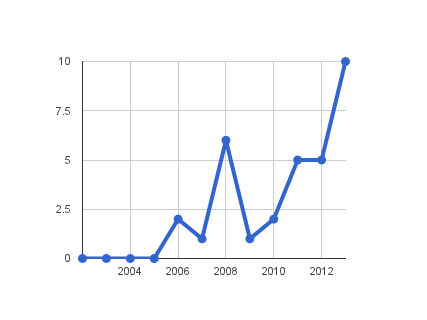
\includegraphics[scale=0.7]{cap3_pub_anuales.png}
  \end{center}
  \caption{Distribución de las publicaciones por años}
  \label{fig:PublicacionesAnuales}
\end{figure}

La revista es el medio en el que más de este tipo de artículos se han publicado, tal y como se puede consultar en la tabla \ref{tab:ResumenForumResultados} y en la figura \ref{fig:PublicacionesTipos} con un 53,1\% del total. Esta información se complementa con la distribución de las publicaciones según el foro en el que han sido publicados y que se muestra en la tabla \ref{tab:DistribucionPublicaciones}. En este se puede comprobar como la mayor parte de las publicaciones están relacionadas con la ingeniería y la educación: World Scientific and Engineering Academy and Society Conferences (WSEAS), IEEE Global Engineering Education Conference (EDUCON), European Journal of Education o Revista Iberoamericana de Tecnologías del Aprendizaje (RITA), entre otras, son las publicaciones que más trabajos han aportado a nuestro trabajo.

\begin{table}[H]
  \begin{center}
  \begin{tabular}{| m{4cm} | c |}
    \hline
    PUBLICATION TYPE & RESULTS\\
    \hline
    \hline 
    Journal & 17 \\
    \hline
    Conference & 10 \\
    \hline
    Chapter & 5 \\
    \hline
  \end{tabular}
\end{center}
\caption{Cantidad de trabajos según el medio en el que fueron publicados}
\label{tab:ResumenForumResultados}
\end{table} 

\begin{figure}[H]
  \begin{center}
    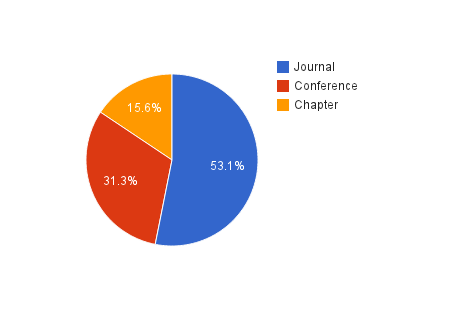
\includegraphics[scale=0.7]{cap3_pub_types.png}
  \end{center}
  \caption{Distribución de publicaciones según el medio en el que fueron publicados}
  \label{fig:PublicacionesTipos}
\end{figure}

\begin{table}[H]
  \begin{center}
  \begin{tabular}{| m{12cm} | c |}
    \hline
    PUBLICATION FORUM & PAPERS\\
    \hline
    \hline 
    World Scientific and Engineering Academy and Society Conferences & 4\\
    \hline
    IEEE Global Engineering Education Conference & 2\\
    \hline
    Australian Society for Computers in Learning in Tertiary Education & 2\\
    \hline
    European Journal of Education & 2\\
    \hline
    Revista Iberoamericana de Tecnologías del Aprendizaje & 2\\
    \hline
    Assessment \& Evaluation in Higher Education & 1\\
    \hline
    Australasian Journal of Educational Technology & 1\\
    \hline
    Conference on Software Engineering Education and Training & 1\\
    \hline
    Competency-based Language Teaching in Higher Education & 1\\
    \hline
    Computers in Human Behavior & 1\\
    \hline
    Computing Colombian Conference & 1\\
    \hline
    Decision Support Systems & 1\\
    \hline
    Game-based learning in higher education and lifelong learning: bridging the gap between theory and practice & 1\\
    \hline
    Human Factors and Ergonomics in Manufacturing \& Service Industries & 1\\
    \hline
    International Conference on Advanced Learning Technologies & 1\\
    \hline
    International Journal of Learning Technology & 1\\
    \hline
    Journal of Computer Assisted Learning & 1\\
    \hline
    Medical Education & 1\\
    \hline
    Revista de Educación & 1\\
    \hline
    The Internet and Higher Education & 1\\
    \hline
    Ubiquitous and Mobile Learning in the Digital Age & 1 \\
    \hline
  \end{tabular}
\end{center}
\caption{Distribución de las publicaciones}
\label{tab:DistribucionPublicaciones}
\end{table} 



\section{Esquema de clasificación y mapeo del estudio}

Una vez revisados todos los artículos se han extraído unas características o categorías comunes a la tipología de los trabajos. Todos los trabajos seleccionados hacen uso de algún tipo de software o metodología para evaluar algún tipo de competencia genérica. Pero ningún trabajo utiliza un enfoque como el que se propone en la introducción de este capítulo, es decir, aprovechando los registros de interacción de los estudiantes con el LMS como indicadores del desempeño de las competencias genéricas. Encontramos trabajos que se apoyan en la tecnología para las competencias pero que terminan delegando parte de la evaluación en el alumno, ya sea mediante autoevaluación o evaluación entre iguales. Otros trabajos se basan en videojuegos o en las redes sociales para evaluar alguna competencia, mientras que otros desarrollan algún tipo de software o técnica. Finalmente hay algunos trabajos que simplemente detectan en su entorno la necesidad de la evaluación de las competencias de manera automática porque su forma de hacerlo les ocasiona una serie de problemas o desventajas con respecto a otro método que proponen o demandan. Además se han encontrado algunas revisiones sobre la literatura relacionadas que también serán tratadas a parte.  En la tabla \ref{tab:PublicacionesForum} se puede ver la distribución de las publicaciones, apoyadas gráficamente en la figura  \ref{fig:PublicacionesForum}.

\begin{table}[H]
  \begin{center}
  \begin{tabular}{| m{4cm} | c |}
    \hline
    PUBLICATION ISSUE & PAPERS\\
    \hline
    \hline 
    Evaluaciones & 11\\
    \hline
    Necesidad & 8\\
    \hline
    Red social & 2\\
    \hline
    Videojuegos & 5\\
    \hline
    Revisiones & 3\\
    \hline
    Técnicas & 8 \\
    \hline
  \end{tabular}
\end{center}
\caption{Distribución de publicaciones por tratamiento del problema}
\label{tab:PublicacionesForum}
\end{table} 

\begin{figure}[H]
  \begin{center}
    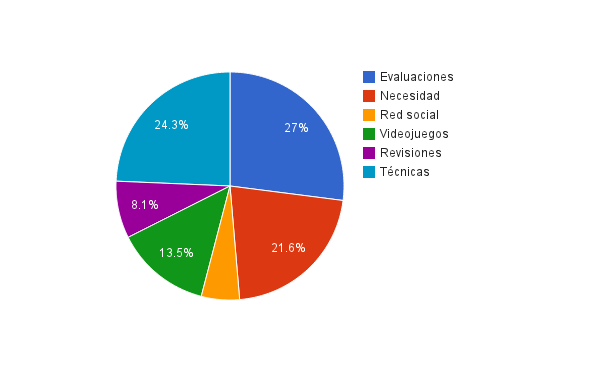
\includegraphics[scale=0.7]{cap3_pub_forum.png}
  \end{center}
  \caption{Distribución de publicaciones por tratamiento del problema}
  \label{fig:PublicacionesForum}
\end{figure}

% Incluir burbujas

\section{Esquema de clasificación}

% Lo dejo aquí. Traer a este esquema de clasificación el reserch scope que puse en el apartado anterior, y en el apartado anterior fijarme en lo que hizo Iván. (Dice algo de step keyworking ...).



En los siguientes apartados, se presentan los resultados del estudio para cada área de investigación. %Los documentos base de este estudio están incluidos en el Apéndice.

\subsection{Metodologías que delegan en los alumnos}
Para favorecer el desarrollo del aprendizaje se utilizan estrategias evaluativas como la autoevaluación, la evaluación entre iguales y la coevaluación. Estas aportan beneficios a estudiantes y profesores universitarios, como la mejora de los procesos y productos del aprendizaje, el desarrollo de estrategias interpersonales, la mejora de la capacidad para emitir juicios o el desarrollo de determinadas competencias académicas y profesionales \cite{Ibarra:2012}. Además, cuando el número de alumnos y la cantidad de información a tener en cuenta en la evaluación crecen, evaluar el trabajo de cada estudiante se vuelve un trabajo muy poco escalable \cite{Balderas:2012}.

Esta estrategia se apoya en el uso de algún tipo de tecnología para trabajar y evaluar una competencia genérica, dejando a posteriori a criterio del alumno la labor de valorar si un compañero o él mismo han alcanzado dicha competencia gracias a la actividad desarrollada. Aunque este enfoque tiene sus beneficios tanto para profesores como para estudiantes, una revisión del profesor podría ser igualmente un trabajo inabarcable.

\subsection{Videojuegos}
Son numerosos los estudios que han tratado las ventajas del aprendizaje basado en juegos (GBL, Game-based learning) \cite{Costu:2009,Munoz:2011}. En estos trabajos se presentan juegos de simulación virtual para cursos que fomentan la colaboración de la universidad y la industria. Juegos que simulan situaciones de la vida real para el desempeño de ciertas competencias y que serán útiles para la industria. Las simulaciones son ambientes de aprendizaje complejos y desafiantes que presentan dificultades para los estudiantes, ya que éstos carecen de una comprensión fundamental de los conceptos específicos del dominio, las relaciones y estrategias de resolución de problemas \cite{Kirkley:2004}. Uno de los factores importantes de esta simulación es la configuración de aprendizaje \cite{Thavikulwat:2010}, la alineación de objetivos, los métodos de aprendizaje y evaluación con los resultados de aprendizaje previstos. Esta evaluación es el aspecto que más nos interesa analizar. Aunque no siempre se realiza de manera automática, sino que a menudo se apoya en el uso de algún tipo de rúbrica facilitada por el LMS.
 
\subsection{Técnicas}
En esta categoría se recogen todos aquellos trabajos que aporten propuestas automáticas o semiautomáticas para la evaluación de competencias genéricas basados en algún modelo. Son herramientas que permiten a los estudiantes, en primer lugar, identificar sus puntos fuertes y débiles y desarrollar estrategias personales para la mejora. En segundo lugar, proporciona a los profesores con información adicional sobre los efectos de su enseñanza en las competencias de los estudiantes. Y por último, proporciona información útil para gestión de la calidad de los programas de enseñanza, ya que puede detectar tendencias en las necesidades de formación de los nuevos estudiantes y ayudar a mejorar el contenido \cite{Achcaoucaou:2012}.

\subsection{Necesidades}
La búsqueda de trabajos relacionados no ha proporcionado muchos resultados directamente relacionados. Sin embargo, aunque no aporten una herramienta concreta, sí hemos encontrado trabajos que detectaban la necesidad de un método, herramienta o modelo para la evaluación de competencias genéricas. Se han añadido a este trabajo los más relevantes de dichos artículos. Este cambio conceptual en el área de la evaluación asistida tiene su motivación en el cambio pedagógico global de conocimiento para el aprendizaje basado en competencias y el reciente énfasis en competencias genéricas, ya que son conscientes de que los cambios en los planes de estudio y en los objetivos del aprendizaje son ineficaces si las prácticas de evaluación siguen siendo las mismas \cite{Cachia:2011, Redecker:2013}.

\subsection{Revisiones}
Con las diferentes revisiones de estado del arte encontradas con respecto a la evaluación de competencias genéricas, se evidencia que hay varios modelos y herramientas para el desarrollo y evaluación de de las mismas, que hacen hincapié en los modelos de datos que soportan los diferentes procesos formativos. Así mismo se plantean modelos de evaluación apoyados en criterios y los niveles de competencia que deben ser valorados por todos los participantes en el proceso de aprendizaje \cite{Cardona:2013}.



\chapter{Respuestas}
En esta sección, se trata de dar respuesta a las preguntas de investigación.

%, a continuación se dan varias ideas que podrían ser extraídas de los resultados del estudio, y después, debatimos algunas de las posibles amenazas a la validez de este trabajo.


\section{Respuestas a preguntas de investigación}
En los artículos de este trabajo se tratan diversas competencias. Unas se trabajan y evalúan, otras sólo se mencionan y otros evalúan competencias no reconocidas como tal. En los siguientes apartados, correspondientes a cada una de las preguntas de investigación, se han separado las respuestas por competencias, indicando qué artículos pueden servir como ejemplo para cada caso. %Hay artículos, que hacen una revisión de trabajos como puede ser \cite{Redecker:2012}.

%-----------
% PREGUNTA 1
%-----------
\subsection{¿Qué competencias se han evaluado de forma automática o asistida por ordenador a partir del uso de los entornos virtuales?}
Las competencias que se han evaluado en los artículos de este trabajo son las siguientes:
\begin{itemize}
\item Capacidad para comunicarse en un segundo idioma \cite{Shih:2011}, \cite{MercedesRico:2013}, \cite{Masip-Alvarez:2013}
\item Capacidad para comunicarse de forma oral y por medio de la palabra escrita en la lengua materna \cite{Mohamed:2008}, \cite{Piedra:2010}, \cite{Liao:2013}, \cite{Masip-Alvarez:2013}, \cite{Colomo-Palacios:2013}
\item Capacidad para generar nuevas ideas (creatividad) \cite{Piedra:2010}, \cite{Liao:2013}, \cite{Colomo-Palacios:2013}
\item Capacidad para trabajar en equipo \cite{McMahon:2007}, \cite{Mohamed:2008}, \cite{Rashid:2008}, \cite{Lim:2011}, \cite{Liao:2013}, \cite{Masip-Alvarez:2013}, \cite{Colomo-Palacios:2013}
\item Capacidad para tomar decisiones razonadas \cite{Achcaoucaou:2012}, \cite{Colomo-Palacios:2013}
\item Capacidad para planificar y administrar el tiempo \cite{Achcaoucaou:2012}, \cite{Liao:2013}
\item Capacidad para adaptarse y actuar en nuevas situaciones \cite{Liao:2013}
\item La apreciación y el respeto por la diversidad y multiculturalidad \cite{Liao:2013}, \cite{Colomo-Palacios:2013}
\item Capacidad de aplicar los conocimientos en situaciones prácticas \cite{Liao:2013}
\item Capacidad para identificar, plantear y resolver problemas \cite{Achcaoucaou:2012}, \cite{Guenaga:2013}, \cite{Colomo-Palacios:2013}
\item Habilidad para trabajar de forma autónoma \cite{Colomo-Palacios:2013}
\item Capacidad para el pensamiento abstracto, análisis y síntesis \cite{Colomo-Palacios:2013}
\item Capacidad para ser críticos y autocríticos \cite{Colomo-Palacios:2013}
\item Espíritu de empresa, la capacidad de tomar la iniciativa \cite{Colomo-Palacios:2013}
\end{itemize}

%-----------
% PREGUNTA 2
%-----------
\subsection{¿Qué herramientas o metodologías se utilizan para evaluar competencias mediante el uso de los entornos virtuales?}
Las herramientas o metodologías que se han empleado en nuestra selección primaria para cada competencia son las siguientes:
\begin{itemize}
\item Capacidad para comunicarse en un segundo idioma:
	\begin{itemize} 
	\item Facebook \cite{Shih:2011}
	\item Second Life \cite{MercedesRico:2013}
	\item Grabación en vídeo \cite{Masip-Alvarez:2013}
	\end{itemize}
\item Capacidad para comunicarse de forma oral y por medio de la palabra escrita en la lengua materna:
	\begin{itemize} 
	\item Grabación en vídeo \cite{Masip-Alvarez:2013}
	\end{itemize}
\item Capacidad para trabajar en equipo:
	\begin{itemize} 
	\item Entorno de seguimiento de trabajo en equipo. JAMTART (Joe And Marks Tracking And Reporting Tool) \cite{McMahon:2007}
	\item Grabación en vídeo \cite{Masip-Alvarez:2013}, \cite{Martin-Cuadrado:2013}
	\item Wikis \cite{Piedra:2010}, \cite{Lim:2011}
	\end{itemize}
\item Capacidad para tomar decisiones razonadas:
	\begin{itemize} 
	\item Tricuspoid \cite{Achcaoucaou:2012}, se trata de una plataforma digital diseñada específicamente para la auto-evaluación de competencias empresariales.
	\end{itemize}
\item Capacidad para planificar y administrar el tiempo
	\begin{itemize} 
	\item Tricuspoid \cite{Achcaoucaou:2012}.
	\end{itemize}
\item Capacidad para generar nuevas ideas (creatividad):
	\begin{itemize} 
	\item Wikis, blogs \cite{Piedra:2010}
	\end{itemize}
\item Capacidad para identificar, plantear y resolver problemas:
	\begin{itemize} 
	\item Tricuspoid \cite{Achcaoucaou:2012}.
	\item Juego serio \cite{Guenaga:2013}
	\end{itemize}
\end{itemize}

%-----------
% PREGUNTA 3
%-----------
\subsection{¿Con qué técnicas se pueden obtener evidencias (numéricas) objetivas del desarrollo de las siguientes competencias en un entorno virtual?}
\begin{itemize}
\item Capacidad para comunicarse en un segundo idioma:
	\begin{itemize} 
	\item Evaluación entre iguales y/o autoevaluación \cite{Shih:2011}, \cite{Masip-Alvarez:2013}
	\item Evaluación conjunta de varios profesores \cite{MercedesRico:2013}
	\end{itemize}
\item Capacidad para comunicarse de forma oral y por medio de la palabra escrita en la lengua materna
	\begin{itemize} 
	\item Autoevaluación \cite{Liao:2013}
	\item Evaluación entre iguales y/o autoevaluación \cite{Masip-Alvarez:2013}
	\item Rúbricas \cite{Mohamed:2008}
	\end{itemize}
\item Capacidad para generar nuevas ideas (creatividad)
	\begin{itemize} 
	\item Autoevaluación \cite{Liao:2013}
	\end{itemize}
\item Capacidad para trabajar en equipo
	\begin{itemize} 
	\item Autoevaluación y/o evaluación entre iguales \cite{McMahon:2007}, \cite{Lim:2011}, \cite{Masip-Alvarez:2013}, \cite{Liao:2013}
	\item Rúbricas \cite{Mohamed:2008}, \cite{Piedra:2010}
	\item Técnica estadística: Modelo ESPEGS \cite{Rashid:2008}
	\end{itemize}
\item Capacidad para tomar decisiones razonadas:
	\begin{itemize} 
	\item Autoevaluación y/o evaluación entre iguales \cite{Achcaoucaou:2012}
	\end{itemize}
\item Capacidad para planificar y administrar el tiempo
	\begin{itemize} 
	\item Autoevaluación y/o evaluación entre iguales \cite{Achcaoucaou:2012}, \cite{Liao:2013}
	\end{itemize}
\item Capacidad para adaptarse y actuar en nuevas situaciones
	\begin{itemize} 
	\item Autoevaluación \cite{Liao:2013}
	\end{itemize}
\item La apreciación y el respeto por la diversidad y multiculturalidad:
	\begin{itemize} 
	\item Autoevaluación \cite{Liao:2013}
	\end{itemize}
\item Capacidad de aplicar los conocimientos en situaciones prácticas:
	\begin{itemize} 
	\item Autoevaluación \cite{Liao:2013}
	\end{itemize}
\item Capacidad para identificar, plantear y resolver problemas:
	\begin{itemize} 
	\item Autoevaluación y/o evaluación entre iguales \cite{Achcaoucaou:2012}
	\item Indicadores basados en rúbrica \cite{Guenaga:2013}
	\end{itemize}
\item Habilidad para trabajar de forma autónoma:
	\begin{itemize} 
	\item Autoevaluación y/o evaluación entre iguales \cite{Colomo-Palacios:2013}
	\end{itemize} 
\item Habilidad para trabajar de forma autónoma:
	\begin{itemize} 
	\item Autoevaluación y/o evaluación entre iguales \cite{Colomo-Palacios:2013}
	\end{itemize} 
\item Capacidad para el pensamiento abstracto, análisis y síntesis:
	\begin{itemize} 
	\item Autoevaluación y/o evaluación entre iguales \cite{Colomo-Palacios:2013}
	\end{itemize} 
\item Capacidad para ser críticos y autocríticos:
	\begin{itemize} 
	\item Autoevaluación y/o evaluación entre iguales \cite{Colomo-Palacios:2013}
	\end{itemize} 
\item Espíritu de empresa, la capacidad de tomar la iniciativa:
	\begin{itemize} 
	\item Autoevaluación y/o evaluación entre iguales \cite{Colomo-Palacios:2013}
	\end{itemize} 
\end{itemize}

%-----------
% PREGUNTA 4
%-----------
\subsection{¿Los resultados que se obtendrían de la evaluación de competencias genéricas de los alumnos mediante el uso de los registros de actividad de los entornos virtuales son indicadores fiables del desempeño de dichas competencias?}

No se han encontrado trabajos que aborden esta problemática de manera directa, aunque sí se han encontrado evidencias en la literatura que puedan ayudar a responder a esta pregunta. En alguno de los trabajos se utilizan wikis para fomentar el desempeño de los alumnos en diferentes competencias \cite{Piedra:2010}. Lim indica que los tutores pueden recoger una gran cantidad de información acerca de sus estudiantes mediante la observación de desempeño de los alumnos, mediante la construcción de los wikis, los comentarios realizados por los estudiantes, y los intercambios entre estudiante \cite{Lim:2011}. Pero es evidente que si el curso tiene un gran número de alumnos la observación se vuelve inabordable. Nuestro trabajo va en la línea de observar el trabajo de los alumnos en los LMS mediante la extracción automática de indicadores. Aunque un LMS es más completo en cuánto al ámbito de actuación que un wiki, en ambos los usuarios trabajan en el sistema de forma independiente, dejando un rastro de su actividad y en ambos se sustenta el trabajo colaborativo. Es más, los LMS suelen incluir un wiki en su estructura. \emph{Un wiki es un tipo de página web que brinda la posibilidad de que multitud de usuarios puedan editar sus contenidos a través del navegador web, con ciertas restricciones mínimas. De esta forma permite que múltiples autores puedan crear, modificar o eliminar los contenidos. Se puede identificar a cada usuario que realiza un cambio y recuperar los contenidos modificados, volviendo a un estado anterior. Estas características facilitan el trabajo en colaboración así como la coordinación de acciones e intercambio de información sin necesidad de estar presentes físicamente ni conectados de forma simultánea} (Wikipedia). 

Por último, Cardona dice que la evaluación de las competencias implica la identificación de los elementos en torno a los procesos de aprendizaje, lo que hace que sea una actividad constante que requiere de criterios para evaluar los resultados durante la formación de las personas \cite{Cardona:2013}. Consideramos que el rastro que dejan los alumnos, su interacción con el entorno, es un reflejo de su trabajo. Chebil indica como se podrían analizar las situaciones que se dan en la aplicación de las tecnologías al aprendizaje (TEL, Technology Enhanced Learning) mediante la recopilación de los rastros de interacción producidos por estos entornos \cite{Chebil:2012}. Mientras que Florian argumenta que para poder utilizar esta información almacenada acerca de las actividades del curso, se requiere filtrado antes de que pueda ser utilizado para procesarla \cite{Florian:2011}.




\chapter{Trabajo (presente y) futuro}
\section{EvalCourse}
En este trabajo hemos buscado literatura que aborde la evaluación de competencias genéricas, y a ser posible, que lo hagan de manera automática utilizando la interacción de los estudiantes con el LMS. En línea con este trabajo, y a fin de abordar lo que será mi futura tesis doctoral, estamos trabajando en una herramienta que cumpla este propósito. Esta herramienta, cuyo prototipo ya ha sido presentado en varios congresos \cite{Balderas:2013,Balderas:2013a}, se llama EvalCourse y su lógica viene descrita en la figura \ref{fig:EvalcourseLogica}. EvalCourse es un Lenguaje de Dominio Específico (DSL). Un DSL es un lenguaje de programación orientado a un problema específico y con una semántica orientada al dominio para el que se diseña. En nuestro caso, este dominio es la evaluación de indicadores de competencias de los estudiantes. Un ejemplo de funcionamiento puede verse en la figura \ref{fig:EvalCourseCodigo}. El objetivo de EvalCourse es ayudar al docente en la evaluación del desempeño de los alumnos en las competencias que éstos deben desarrollar a lo largo del curso. Estos datos deberán servir al docente como indicadores del desarrollo de dichas competencias. La idea inicial con la que se ha desarrollado este proyecto, es que el DSL sea genérico y pueda ser utilizado con otros sistemas, no sólo de tipo LMS, sino también con sistemas que fomenten el trabajo colaborativo, como pueden ser los wikis. De hecho, se ha desarrollado software para evaluar diversas competencias (tanto genéricas como específicas) mediante análisis de registro (StatMediaWiki) como entre pares o autoevaluaciones (AssessMediaWiki) \cite{Palomo-Duarte:2013}.



\begin{figure}[H]
  \begin{center}
    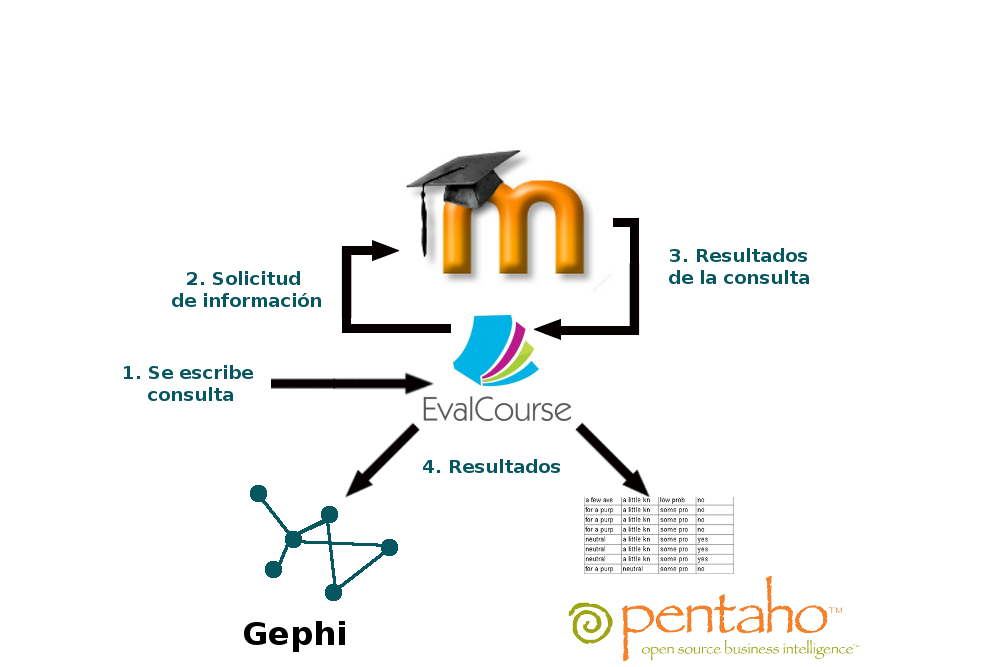
\includegraphics[scale=0.25]{cap5_evalcourse_logica.png}
  \end{center}
  \caption{Esquema lógico de EvalCourse}
  \label{fig:EvalcourseLogica}
\end{figure}


\begin{figure}[H]
  \begin{center}
    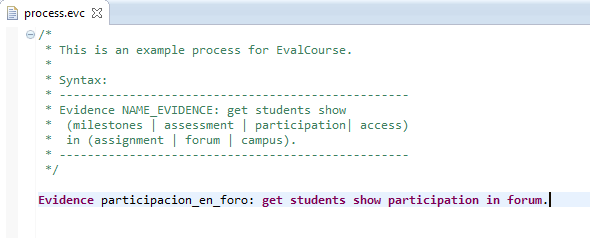
\includegraphics[scale=0.6]{cap5_evalcourse_codigo.png}
  \end{center}
  \caption{Consulta realizada en EvalCourse para obtener la participación en foros}
  \label{fig:EvalCourseCodigo}
\end{figure}

\section{Experiencia piloto}
Durante el presente curso 2013/14 se está desarrollando un proyecto financiado por la Convocatoria de Actuaciones Avaladas para la Mejora Docente, Formación del Profesorado y Difusión de Resultados con fondos de la Consejería de Economía, Innovación, Ciencia y Empleo de la Junta de Andalucía, con el título \emph{Extracción de indicadores objetivos para evaluación del desarrollo de competencias genéricas a partir de registros de actividad del Campus Virtual}. La Unidad de Innovación Docente de la Universidad de Cádiz concedió dicha actuación con código \emph{AAA\_14\_009} y actualmente se está desarrollando. En ella participan 8 profesores de 6 asignaturas del Grado en Ingeniería Informática.

Este proyecto se engloba dentro del trabajo realizado dentro del grupo de investigación SPI\&FM (TIC-195) por parte de Antonio Balderas al uso de las tecnologías en los entornos de aprendizaje. Se pretende desarrollar y aplicar EvalCourse, un DSL que permita a los docentes mediante el uso de una sintaxis sencilla obtener indicadores del desempeño de los estudiantes en diferentes competencias. Son varias las asignaturas de Grado en Ingeniería Informática que participan en este proyecto. Las tareas que comprende son:

\begin{enumerate}
\item Analizar los tipos de indicadores que se podrían obtener de la base de datos Moodle que sean de utilidad para los profesores, así como la manera de obtenerlos.
\item Análisis, desarrollo y prueba del software. Implementar el software DSL para que se conecte a Moodle y pueda extraer la información. Para ello sería necesario la instalación de un entorno de pruebas Moodle y la generación de una batería de datos de pruebas que permita verificar el funcionamiento del software.
\item Obtención de datos reales de las asignaturas del campus virtual. A partir de estos, utilizaremos la herramienta para obtener todos los indicadores necesarios para evaluar las competencias de los estudiantes. Además podremos corregir aquellos fallos que se detecten en el software.
\item Análisis de resultados de la experiencia, difusión del trabajo realizado, publicación de informes, correcciones menores en el sistema, etc. Se analizarán los resultados obtenidos y se darán a conocer el software y la experiencia en webs especializadas, redes sociales, etc. Igualmente se procederá a la correcta documentación del sistema en una web oficial para poder replicar la experiencia (incidiendo en cómo evitar los errores cometidos), así como pequeños desarrollos que corrijan deficiencias observadas y faciliten la reutilización del sistema.
\end{enumerate}

\section{Trabajo futuro} % Creada sección debido a comentario 89, pero hay que cambiar más. Esperar comentarios Juanma.
El trabajo futuro no es otro que afrontar el desarrollo de mi tesis doctoral. Partimos de las bases sentadas en este trabajo de investigación, habiendo analizado la situación actual de la evaluación de competencias genéricas. Los próximos pasos de esta línea, pasan por seleccionar, por un lado, varios entornos virtuales. Pero estos entornos virtuales ya no serán sólo en Moodle, como han sido las experiencias piloto desarrolladas en los artículos \cite{Balderas:2013,Balderas:2013a}, sino ampliar a otros LMS, a wikis y CMS (Content content Management System). Ya en el curso pasado se realizó una experiencia basada en \emph{AssessMediaWiki} \cite{Balderas:2012}, en el que se utilizaban los registros de un wiki basado en \emph{MediaWiki} para que, mediante evaluación entre iguales, los estudiantes analizasen las diferencias entre los trabajos de dos compañeros. Por tanto, y aunque con otro fin, ya se ha realizado una inmersión a la extracción de datos a partir de los registros del wiki.

Por otro lado, el trabajo futuro se ha de probar con diferentes cursos que cuenten con un alto número de estudiantes, demostrando que este método de evaluación es sostenible, y que además, el método no sufre al incrementar la cantidad de alumnos, validando así su escalabilidad.

Desglosando el párrafo anterior, nos encontramos ante un doble objetivo general como trabajo futuro:
\begin{itemize}
\item Objetivo funcional: ser capaz de recoger información de una diversidad de sistemas: LMS, wikis y CMS.
\item Objetivo no funcional: ser capaz de evaluar el desempeño de los alumnos en el sistema, a pesar de que el número de alumnos sea muy elevado.
\end{itemize}





\chapter{Conclusiones}
% -*-cap1.tex-*-
% Este fichero es parte de la plantilla LaTeX para
% la realización de Proyectos Final de Carrera, protejido
% bajo los términos de la licencia GFDL.
% Para más información, la licencia completa viene incluida en el
% fichero fdl-1.3.tex

% Copyright (C) 2009 Pablo Recio Quijano 

%\section{Introducción}

En el presente documento se ha realizado una revisión formal de la literatura para responder a las preguntas de la investigación relacionadas con la evaluación automatizada de competencias genéricas mediante el uso de entornos de aprendizaje virtuales. Esta revisión formal se ha desarrollado siguiendo las directrices publicadas en la metodología propuesta por Kitchenham.

Se identificaron los términos que se utilizarían en las principales bibliotecas digitales y se realizó la búsqueda para hallar trabajos que ayudasen a responder a las preguntas de investigación que se plantearon. Los criterios de inclusión de artículos nos dejaron un 7\% de los que fueron preseleccionados tras este proceso de búsqueda. La selección primaria ha sido clasificada en base al tipo de contribución que realizan a la ciencia, en base al tipo de investigación y en base al ámbito de aplicación del trabajo. Esta clasificación ha sido representada mediante diferentes tablas y figuras.

El escaso número de resultados obtenido viene a corroborar la escasez de colaboraciones entre ciencias de la educación e informática. El grueso de artículos rescatado data de los últimos 3 años. De los trabajos encontrados, la tendencia dominante con un 43,8\% es la de delegar en el alumno, ya sea mediante autoevaluación, o mediante evaluación entre iguales, la corrección de las actividades que evidencian el desempeño de una competencia. Además, la segunda tendencia, con un 21,9\% es la que se basa en rúbricas para refrendarlo. Al final, este método también delega en una persona o conjunto de personas, sólo que esta vez es el profesor el encargado de corregirlo. Es decir, un 65,7\% de los trabajos encontrados necesita de la intervención humana para calcular las puntuaciones, por lo que el procedimiento no es automático, lo que de algún u otro modo, podría incurrir en tareas no escalables para el docente.

Por otro lado, están las herramientas GBL, con un 18,8\%, que aunque automatizan la evaluación del desempeño en el juego de un alumno, no están integradas con el sistema de evaluación, por lo que traspasar las notas a la plataforma de la asignatura es una tarea que de nuevo implica al docente. Finalmente, queda un 15,6\% de trabajos de diversa índole, en los que se combinan herramientas para la evaluación de competencias y se realizan revisiones de otros trabajos.

Estos trabajos se utilizaron para responder a cada una de las preguntas de investigación. Como se indicaba en el párrafo anterior, los trabajos encontrados evalúan competencias genéricas, aunque no lo hacen desde una perspectiva tan automatizada como se pretende que sea nuestro trabajo.

Se presentan las líneas de trabajo futuro, basadas en el desarrollo de la herramienta EvalCourse para la evaluación automática de indicadores de los LMS. En la actualidad hay un proyecto de Innovación Docente coordinado por el autor de este trabajo y que junto con este trabajo forman las bases de la que será su tesis doctoral.






%\chapter{Desarrollo del proyecto}
%% -*-cap2.tex-*-
% Este fichero es parte de la plantilla LaTeX para
% la realización de Proyectos Final de Carrera, protejido
% bajo los términos de la licencia GFDL.
% Para más información, la licencia completa viene incluida en el
% fichero fdl-1.3.tex

% Copyright (C) 2009 Pablo Recio Quijano 

\section{Organización temporal}

En este apartado podemos añadir un diagrama de Gannt, con la
planificación temporal que se realizó del proyecto. Para ello podemos
usar algún programa libre como por ejemplo \programa{Planner}:

\figura{gannt.png}{scale=0.6}{Diagrama de Gannt. Desarrollo del
  proyecto}{gannt}{H}

Observad el código, notareis algo distinto con respecto a las imágenes
del capítulo anterior. En este caso utilizo un comando personalizado
en \comando{comandos.sty}, donde simplifico la creación de una
figura, como en la figura~\ref{gannt}. % Podemos poner o no la ~

\section{Análisis del sistema}

Si el proyecto se refiere a un sistema software, normalmente
procederemos a un análisis y a un diseño del sistema usando notación
UML, para organizar correctamente dicho sistema.\\

\LaTeX{} no trae soporte nativo para hacer este tipo de diagramas, y
aunque se pueden utilizar paquetes que lo hagan. Sin embargo lo más
cómodo es que utilizemos herramientas CASE para ayudarnos a dicha
tarea, como pueden ser \programa{Dia} o \programa{Umbrello}, como
podemos ver en la figura \ref{uml}.

\figura{uml.png}{scale=1}{UML de ejemplo con Umbrello}{uml}{H}

Ya que no es el objetivo de este documento trabajar con dichas
herramientas, aprovecharé este apartado para mostrar algunas
cosas más de las que podemos dotar a nuestro documento \LaTeX{}.\\

Sabemos que tenemos un fichero \texttt{bibliografia.bib}, para que la
herramienta Bib\TeX{}  nos genere las referencias bibliográficas. Sin
embargo a priori no se mostrarán hasta que nos las referenciemos.\\

Teniendo en cuenta que todo esto lo tomamos desde la ``biblia'' de
\LaTeX, podemos hacer una referencia a ella \cite{mitt04}. También hay
que saber que una guia de referencia online muy buena es la página en
\texttt{wikibooks} de \LaTeX{} \cite{website:latex-wikibooks}. 

% TO-DO: Multirow, Multicolumn y Supertabular.

\section{Base de Datos}

Supongamos que en este apartado, queremos incluir un \negrita{diagrama
Entidad-Relación Extendido}, que modele la base de datos que vamos a
utilizar en nuestro proyecto. Una posible herramienta para dibujarla
es \programa{Dia}, una herramienta pra gráficos vectoriales bastante
completa. Una vez hemos hecho el diagrama, podemos importarlo a una
imagen en multitud de formatos, o también podemos a código
\programa{.tex}.\\

¿Qué utilidad tiene esto? Pues basicamente lo podremos modificar para
refinarlo un poco, añadirle fórmulas matemáticas si quisieramos, o
diversas cosas. Además de comprimir bastante en espacio respecto a una
imagen. El diagrama \ref{ERe}, está realizado con Dia importándolo a
\LaTeX{}:

\begin{figure}[H]
  \label{ERe}
  \begin{center}
    % -*-ERe.tex-*-
% Este fichero es parte de la plantilla LaTeX para
% la realización de Proyectos Final de Carrera, protejido
% bajo los términos de la licencia GFDL.
% Para más información, la licencia completa viene incluida en el
% fichero fdl-1.3.tex

% Copyright (C) 2009 Pablo Recio Quijano, Noelia Sales Montes

% necesita \usepackage{tikz}
\ifx\du\undefined
  \newlength{\du}
\fi
\setlength{\du}{15\unitlength}
\begin{tikzpicture}
\pgftransformxscale{1.000000}
\pgftransformyscale{-1.000000}
\definecolor{dialinecolor}{rgb}{0.000000, 0.000000, 0.000000}
\pgfsetstrokecolor{dialinecolor}
\definecolor{dialinecolor}{rgb}{1.000000, 1.000000, 1.000000}
\pgfsetfillcolor{dialinecolor}
\definecolor{dialinecolor}{rgb}{1.000000, 1.000000, 1.000000}
\pgfsetfillcolor{dialinecolor}
\fill (20.800000\du,-5.900000\du)--(20.800000\du,-3.900000\du)--(25.475000\du,-3.900000\du)--(25.475000\du,-5.900000\du)--cycle;
\pgfsetlinewidth{0.100000\du}
\pgfsetdash{}{0pt}
\pgfsetmiterjoin
\definecolor{dialinecolor}{rgb}{0.000000, 0.000000, 0.000000}
\pgfsetstrokecolor{dialinecolor}
\draw (20.800000\du,-5.900000\du)--(20.800000\du,-3.900000\du)--(25.475000\du,-3.900000\du)--(25.475000\du,-5.900000\du)--cycle;
% setfont left to latex
\definecolor{dialinecolor}{rgb}{0.000000, 0.000000, 0.000000}
\pgfsetstrokecolor{dialinecolor}
\node at (23.137500\du,-4.597500\du){Empleado};
\definecolor{dialinecolor}{rgb}{1.000000, 1.000000, 1.000000}
\pgfsetfillcolor{dialinecolor}
\fill (20.840000\du,-0.530000\du)--(20.840000\du,1.470000\du)--(25.542500\du,1.470000\du)--(25.542500\du,-0.530000\du)--cycle;
\pgfsetlinewidth{0.100000\du}
\pgfsetdash{}{0pt}
\pgfsetmiterjoin
\definecolor{dialinecolor}{rgb}{0.000000, 0.000000, 0.000000}
\pgfsetstrokecolor{dialinecolor}
\draw (20.840000\du,-0.530000\du)--(20.840000\du,1.470000\du)--(25.542500\du,1.470000\du)--(25.542500\du,-0.530000\du)--cycle;
% setfont left to latex
\definecolor{dialinecolor}{rgb}{0.000000, 0.000000, 0.000000}
\pgfsetstrokecolor{dialinecolor}
\node at (23.191250\du,0.772500\du){Secretaria};
\definecolor{dialinecolor}{rgb}{1.000000, 1.000000, 1.000000}
\pgfsetfillcolor{dialinecolor}
\fill (10.030000\du,-0.510000\du)--(10.030000\du,1.490000\du)--(13.980000\du,1.490000\du)--(13.980000\du,-0.510000\du)--cycle;
\pgfsetlinewidth{0.100000\du}
\pgfsetdash{}{0pt}
\pgfsetmiterjoin
\definecolor{dialinecolor}{rgb}{0.000000, 0.000000, 0.000000}
\pgfsetstrokecolor{dialinecolor}
\draw (10.030000\du,-0.510000\du)--(10.030000\du,1.490000\du)--(13.980000\du,1.490000\du)--(13.980000\du,-0.510000\du)--cycle;
% setfont left to latex
\definecolor{dialinecolor}{rgb}{0.000000, 0.000000, 0.000000}
\pgfsetstrokecolor{dialinecolor}
\node at (12.005000\du,0.792500\du){Monitor};
\definecolor{dialinecolor}{rgb}{1.000000, 1.000000, 1.000000}
\pgfsetfillcolor{dialinecolor}
\fill (30.822600\du,-0.595000\du)--(30.822600\du,1.405000\du)--(36.982600\du,1.405000\du)--(36.982600\du,-0.595000\du)--cycle;
\pgfsetlinewidth{0.100000\du}
\pgfsetdash{}{0pt}
\pgfsetmiterjoin
\definecolor{dialinecolor}{rgb}{0.000000, 0.000000, 0.000000}
\pgfsetstrokecolor{dialinecolor}
\draw (30.822600\du,-0.595000\du)--(30.822600\du,1.405000\du)--(36.982600\du,1.405000\du)--(36.982600\du,-0.595000\du)--cycle;
% setfont left to latex
\definecolor{dialinecolor}{rgb}{0.000000, 0.000000, 0.000000}
\pgfsetstrokecolor{dialinecolor}
\node at (33.902600\du,0.707500\du){Mantenimiento};
\definecolor{dialinecolor}{rgb}{1.000000, 1.000000, 1.000000}
\pgfsetfillcolor{dialinecolor}
\fill (32.354000\du,6.245200\du)--(32.354000\du,8.245200\du)--(35.431500\du,8.245200\du)--(35.431500\du,6.245200\du)--cycle;
\pgfsetlinewidth{0.100000\du}
\pgfsetdash{}{0pt}
\pgfsetmiterjoin
\definecolor{dialinecolor}{rgb}{0.000000, 0.000000, 0.000000}
\pgfsetstrokecolor{dialinecolor}
\draw (32.354000\du,6.245200\du)--(32.354000\du,8.245200\du)--(35.431500\du,8.245200\du)--(35.431500\du,6.245200\du)--cycle;
% setfont left to latex
\definecolor{dialinecolor}{rgb}{0.000000, 0.000000, 0.000000}
\pgfsetstrokecolor{dialinecolor}
\node at (33.892750\du,7.547700\du){Zona};
\definecolor{dialinecolor}{rgb}{1.000000, 1.000000, 1.000000}
\pgfsetfillcolor{dialinecolor}
\fill (26.282700\du,4.070200\du)--(26.282700\du,6.070200\du)--(29.570200\du,6.070200\du)--(29.570200\du,4.070200\du)--cycle;
\pgfsetlinewidth{0.100000\du}
\pgfsetdash{}{0pt}
\pgfsetmiterjoin
\definecolor{dialinecolor}{rgb}{0.000000, 0.000000, 0.000000}
\pgfsetstrokecolor{dialinecolor}
\draw (26.282700\du,4.070200\du)--(26.282700\du,6.070200\du)--(29.570200\du,6.070200\du)--(29.570200\du,4.070200\du)--cycle;
% setfont left to latex
\definecolor{dialinecolor}{rgb}{0.000000, 0.000000, 0.000000}
\pgfsetstrokecolor{dialinecolor}
\node at (27.926450\du,5.372700\du){Socio};
\pgfsetlinewidth{0.100000\du}
\pgfsetdash{}{0pt}
\pgfsetdash{}{0pt}
\pgfsetbuttcap
{
\definecolor{dialinecolor}{rgb}{0.000000, 0.000000, 0.000000}
\pgfsetfillcolor{dialinecolor}
% was here!!!
\definecolor{dialinecolor}{rgb}{0.000000, 0.000000, 0.000000}
\pgfsetstrokecolor{dialinecolor}
\draw (23.178300\du,-0.580358\du)--(23.137500\du,-3.900000\du);
}
\definecolor{dialinecolor}{rgb}{0.000000, 0.000000, 0.000000}
\pgfsetstrokecolor{dialinecolor}
\draw (23.178300\du,-0.580358\du)--(23.145019\du,-3.288243\du);
\pgfsetmiterjoin
\definecolor{dialinecolor}{rgb}{1.000000, 1.000000, 1.000000}
\pgfsetfillcolor{dialinecolor}
\fill (23.395000\du,-3.291315\du)--(23.138874\du,-3.788205\du)--(22.895038\du,-3.285170\du)--cycle;
\pgfsetlinewidth{0.100000\du}
\pgfsetdash{}{0pt}
\pgfsetmiterjoin
\definecolor{dialinecolor}{rgb}{0.000000, 0.000000, 0.000000}
\pgfsetstrokecolor{dialinecolor}
\draw (23.395000\du,-3.291315\du)--(23.138874\du,-3.788205\du)--(22.895038\du,-3.285170\du)--cycle;
\pgfsetlinewidth{0.100000\du}
\pgfsetdash{}{0pt}
\pgfsetdash{}{0pt}
\pgfsetmiterjoin
\pgfsetbuttcap
{
\definecolor{dialinecolor}{rgb}{0.000000, 0.000000, 0.000000}
\pgfsetfillcolor{dialinecolor}
% was here!!!
{\pgfsetcornersarced{\pgfpoint{0.000000\du}{0.000000\du}}\definecolor{dialinecolor}{rgb}{0.000000, 0.000000, 0.000000}
\pgfsetstrokecolor{dialinecolor}
\draw (33.902600\du,-0.595000\du)--(33.902600\du,-1.839800\du)--(12.005000\du,-1.839800\du)--(12.005000\du,-0.559434\du);
}}
\definecolor{dialinecolor}{rgb}{1.000000, 1.000000, 1.000000}
\pgfsetfillcolor{dialinecolor}
\fill (9.754000\du,3.791450\du)--(11.972750\du,2.460200\du)--(14.191500\du,3.791450\du)--(11.972750\du,5.122700\du)--cycle;
\pgfsetlinewidth{0.100000\du}
\pgfsetdash{}{0pt}
\pgfsetmiterjoin
\definecolor{dialinecolor}{rgb}{0.000000, 0.000000, 0.000000}
\pgfsetstrokecolor{dialinecolor}
\draw (9.754000\du,3.791450\du)--(11.972750\du,2.460200\du)--(14.191500\du,3.791450\du)--(11.972750\du,5.122700\du)--cycle;
% setfont left to latex
\definecolor{dialinecolor}{rgb}{0.000000, 0.000000, 0.000000}
\pgfsetstrokecolor{dialinecolor}
\node[anchor=east] at (9.454000\du,3.491450\du){};
\definecolor{dialinecolor}{rgb}{0.000000, 0.000000, 0.000000}
\pgfsetstrokecolor{dialinecolor}
\node[anchor=west] at (14.491500\du,3.491450\du){};
\definecolor{dialinecolor}{rgb}{0.000000, 0.000000, 0.000000}
\pgfsetstrokecolor{dialinecolor}
\node at (11.972750\du,4.093950\du){imparte};
\pgfsetlinewidth{0.100000\du}
\pgfsetdash{}{0pt}
\pgfsetdash{}{0pt}
\pgfsetbuttcap
{
\definecolor{dialinecolor}{rgb}{0.000000, 0.000000, 0.000000}
\pgfsetfillcolor{dialinecolor}
% was here!!!
\definecolor{dialinecolor}{rgb}{0.000000, 0.000000, 0.000000}
\pgfsetstrokecolor{dialinecolor}
\draw (11.987836\du,1.538593\du)--(11.972750\du,2.460200\du);
}
\pgfsetlinewidth{0.100000\du}
\pgfsetdash{}{0pt}
\pgfsetdash{}{0pt}
\pgfsetbuttcap
{
\definecolor{dialinecolor}{rgb}{0.000000, 0.000000, 0.000000}
\pgfsetfillcolor{dialinecolor}
% was here!!!
\definecolor{dialinecolor}{rgb}{0.000000, 0.000000, 0.000000}
\pgfsetstrokecolor{dialinecolor}
\draw (11.970796\du,5.169007\du)--(11.968437\du,6.832059\du);
}
\definecolor{dialinecolor}{rgb}{1.000000, 1.000000, 1.000000}
\pgfsetfillcolor{dialinecolor}
\fill (18.404000\du,5.147700\du)--(21.466500\du,3.310200\du)--(24.529000\du,5.147700\du)--(21.466500\du,6.985200\du)--cycle;
\pgfsetlinewidth{0.100000\du}
\pgfsetdash{}{0pt}
\pgfsetmiterjoin
\definecolor{dialinecolor}{rgb}{0.000000, 0.000000, 0.000000}
\pgfsetstrokecolor{dialinecolor}
\draw (18.404000\du,5.147700\du)--(21.466500\du,3.310200\du)--(24.529000\du,5.147700\du)--(21.466500\du,6.985200\du)--cycle;
% setfont left to latex
\definecolor{dialinecolor}{rgb}{0.000000, 0.000000, 0.000000}
\pgfsetstrokecolor{dialinecolor}
\node[anchor=east] at (18.104000\du,4.847700\du){};
\definecolor{dialinecolor}{rgb}{0.000000, 0.000000, 0.000000}
\pgfsetstrokecolor{dialinecolor}
\node[anchor=west] at (24.829000\du,4.847700\du){};
\definecolor{dialinecolor}{rgb}{0.000000, 0.000000, 0.000000}
\pgfsetstrokecolor{dialinecolor}
\node at (21.466500\du,5.450200\du){apuntado en};
\pgfsetlinewidth{0.100000\du}
\pgfsetdash{}{0pt}
\pgfsetdash{}{0pt}
\pgfsetbuttcap
{
\definecolor{dialinecolor}{rgb}{0.000000, 0.000000, 0.000000}
\pgfsetfillcolor{dialinecolor}
% was here!!!
\definecolor{dialinecolor}{rgb}{0.000000, 0.000000, 0.000000}
\pgfsetstrokecolor{dialinecolor}
\draw (24.529000\du,5.147700\du)--(26.232300\du,5.108850\du);
}
\pgfsetlinewidth{0.100000\du}
\pgfsetdash{}{0pt}
\pgfsetdash{}{0pt}
\pgfsetmiterjoin
\pgfsetbuttcap
{
\definecolor{dialinecolor}{rgb}{0.000000, 0.000000, 0.000000}
\pgfsetfillcolor{dialinecolor}
% was here!!!
{\pgfsetcornersarced{\pgfpoint{0.000000\du}{0.000000\du}}\definecolor{dialinecolor}{rgb}{0.000000, 0.000000, 0.000000}
\pgfsetstrokecolor{dialinecolor}
\draw (11.966970\du,8.929609\du)--(11.967000\du,10.550000\du)--(33.892750\du,10.550000\du)--(33.892750\du,8.245200\du);
}}
\definecolor{dialinecolor}{rgb}{1.000000, 1.000000, 1.000000}
\pgfsetfillcolor{dialinecolor}
\fill (20.900700\du,10.539700\du)--(23.908200\du,8.735200\du)--(26.915700\du,10.539700\du)--(23.908200\du,12.344200\du)--cycle;
\pgfsetlinewidth{0.100000\du}
\pgfsetdash{}{0pt}
\pgfsetmiterjoin
\definecolor{dialinecolor}{rgb}{0.000000, 0.000000, 0.000000}
\pgfsetstrokecolor{dialinecolor}
\draw (20.900700\du,10.539700\du)--(23.908200\du,8.735200\du)--(26.915700\du,10.539700\du)--(23.908200\du,12.344200\du)--cycle;
% setfont left to latex
\definecolor{dialinecolor}{rgb}{0.000000, 0.000000, 0.000000}
\pgfsetstrokecolor{dialinecolor}
\node[anchor=east] at (20.600700\du,10.239700\du){};
\definecolor{dialinecolor}{rgb}{0.000000, 0.000000, 0.000000}
\pgfsetstrokecolor{dialinecolor}
\node[anchor=west] at (27.215700\du,10.239700\du){};
\definecolor{dialinecolor}{rgb}{0.000000, 0.000000, 0.000000}
\pgfsetstrokecolor{dialinecolor}
\node at (23.908200\du,10.842200\du){realizada en};
\pgfsetlinewidth{0.100000\du}
\pgfsetdash{}{0pt}
\pgfsetdash{}{0pt}
\pgfsetbuttcap
{
\definecolor{dialinecolor}{rgb}{0.000000, 0.000000, 0.000000}
\pgfsetfillcolor{dialinecolor}
% was here!!!
\definecolor{dialinecolor}{rgb}{0.000000, 0.000000, 0.000000}
\pgfsetstrokecolor{dialinecolor}
\draw (33.902600\du,1.405000\du)--(33.894521\du,6.195076\du);
}
\definecolor{dialinecolor}{rgb}{1.000000, 1.000000, 1.000000}
\pgfsetfillcolor{dialinecolor}
\fill (9.753200\du,6.880200\du)--(9.753200\du,8.880200\du)--(14.180700\du,8.880200\du)--(14.180700\du,6.880200\du)--cycle;
\pgfsetlinewidth{0.100000\du}
\pgfsetdash{}{0pt}
\pgfsetmiterjoin
\definecolor{dialinecolor}{rgb}{0.000000, 0.000000, 0.000000}
\pgfsetstrokecolor{dialinecolor}
\draw (9.753200\du,6.880200\du)--(9.753200\du,8.880200\du)--(14.180700\du,8.880200\du)--(14.180700\du,6.880200\du)--cycle;
% setfont left to latex
\definecolor{dialinecolor}{rgb}{0.000000, 0.000000, 0.000000}
\pgfsetstrokecolor{dialinecolor}
\node at (11.966950\du,8.182700\du){Actividad};
\pgfsetlinewidth{0.100000\du}
\pgfsetdash{}{0pt}
\pgfsetdash{}{0pt}
\pgfsetmiterjoin
\pgfsetbuttcap
{
\definecolor{dialinecolor}{rgb}{0.000000, 0.000000, 0.000000}
\pgfsetfillcolor{dialinecolor}
% was here!!!
{\pgfsetcornersarced{\pgfpoint{0.000000\du}{0.000000\du}}\definecolor{dialinecolor}{rgb}{0.000000, 0.000000, 0.000000}
\pgfsetstrokecolor{dialinecolor}
\draw (14.231000\du,7.880200\du)--(16.294100\du,7.880200\du)--(16.294100\du,5.147700\du)--(18.357300\du,5.147700\du);
}}
% setfont left to latex
\definecolor{dialinecolor}{rgb}{0.000000, 0.000000, 0.000000}
\pgfsetstrokecolor{dialinecolor}
\node[anchor=west] at (12.450000\du,2.368750\du){1..*};
% setfont left to latex
\definecolor{dialinecolor}{rgb}{0.000000, 0.000000, 0.000000}
\pgfsetstrokecolor{dialinecolor}
\node[anchor=west] at (34.285000\du,2.331250\du){1..*};
% setfont left to latex
\definecolor{dialinecolor}{rgb}{0.000000, 0.000000, 0.000000}
\pgfsetstrokecolor{dialinecolor}
\node[anchor=west] at (34.220000\du,5.516250\du){1..*};
% setfont left to latex
\definecolor{dialinecolor}{rgb}{0.000000, 0.000000, 0.000000}
\pgfsetstrokecolor{dialinecolor}
\node[anchor=west] at (12.255000\du,9.713750\du){1..*};
% setfont left to latex
\definecolor{dialinecolor}{rgb}{0.000000, 0.000000, 0.000000}
\pgfsetstrokecolor{dialinecolor}
\node[anchor=west] at (12.550100\du,6.331250\du){1..*};
% setfont left to latex
\definecolor{dialinecolor}{rgb}{0.000000, 0.000000, 0.000000}
\pgfsetstrokecolor{dialinecolor}
\node[anchor=west] at (24.425000\du,6.133750\du){0..*};
% setfont left to latex
\definecolor{dialinecolor}{rgb}{0.000000, 0.000000, 0.000000}
\pgfsetstrokecolor{dialinecolor}
\node[anchor=west] at (14.560000\du,8.768750\du){1..*};
% setfont left to latex
\definecolor{dialinecolor}{rgb}{0.000000, 0.000000, 0.000000}
\pgfsetstrokecolor{dialinecolor}
\node[anchor=west] at (34.180000\du,9.238750\du){1};
\end{tikzpicture}

    % Comentar si no está el paquete tkiz instalado, y descomentar la
    % linea siguiente. Comentar además la inclusión del paquete en
    % estilos/estiloBase.sty
    %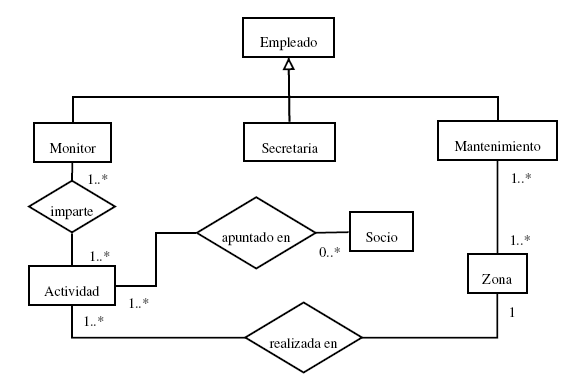
\includegraphics[scale=0.8]{ERe.png}
  \end{center}
  \caption{Diagrama ERe de ejemplo}
\end{figure}


\section{Código fuente}

En \LaTeX tenemos varias maneras de colocar nuestro código fuente, pero
vamos a mostrar dos básicas.

\subsection{Entorno \texttt{Verbatim}}

Este entorno, nos permite incluir dentro de él \negrita{cualquier}
código, y nos respetará espacios, saltos de lineas, tabuladores... es
decir, el compilador de \LaTeX no procesará ese entorno y lo dejará
tal cual está. Veamos un ejemplo con el clásico programa
\programa{Hola mundo} en \texttt{C++}:

\begin{verbatim}
/*Clásico programa en su versión C++*/

#include <iostream>

using namespace std;

int main()
{
  cout << "¡Hola, mundo!" << endl;
  return 0; //No hace falta, pero en fin
}
\end{verbatim}

Vemos, que queda un poco ``soso'': no remarca palabras del lenguaje,
le da igual lo que es comentario y lo que es texto, y claro, a la hora
de tener un código relativamente amplio, pues es incomodo verlo tan
plano. Hay alternativas como \texttt{fncyverbatim}, en la cual podemos
formatearlo algo, añadiendo números de lineas, remarcando palabras del
lenguaje y más opciones, pero quizás la siguiente opción sea más
completa:

\subsection{Entorno \texttt{listing}}

Si vemos en el fichero \comando{comandos.sty}, podemos ver varios
estilos definidos para este entorno. ¿En qué consiste? Pues realmente
este entorno, sabiendo de que lenguaje le estamos pasando el código
(admitiendo gran variedad como C, C++, Java, \TeX, SQL, ADA, Python y
muchísimos más), y ciertas opciones, podemos formatear el código.\\

Este entorno podemos llamarlo de dos formas distintas, la primera es
utilizando un entorno propiamente dicho, con sus
$\backslash$\texttt{begin} y $\backslash$\texttt{end} dentro del cual
copiamos el código, y otra usando el comando
$\backslash$\texttt{lstinputlisting}, pasándole de parámetro el propio
fichero. Veamos de las dos formas:

\begin{lstlisting}[style=C++]
/*Clasico programa en su version C++*/

#include <iostream>

using namespace std;

int main()
{
  cout << "Hola, mundo!" << endl;
  return 0; //No hace falta, pero en fin
}  
\end{lstlisting}

O de la segunda forma:

\lstinputlisting[style=C++]{hola_mundo.cpp}

Notar que uso el estilo \texttt{C++} porque ya lo tengo definido en el
fichero mencionado anteriormente, pero se pueden añadir varios más,
modificando los colores, si queremos o no número de lineas, o por
ejemplo comandos de consola:

\begin{lstlisting}[style=consola]
  g++ hola_mundo.cpp -o hola_mundo
\end{lstlisting}

Desde luego, es bastante más agradable para la vista, lo cual facilita
si lectura. Sin embargo, si usamos esta última opción probablemente
tengamos problemas con los caracteres españoles, acentos y demás,
debido a las diferencias de codificación entre ISO Latin-1 y UTF8. Hay
que tener cuidado en tenerlo todo en UTF8 para que el compilador
``entienda'' los caracteres.

\backmatter % Apéndices, bibliografia ...


\clearpage
\addcontentsline{toc}{chapter}{Bibliografia y referencias}
\bibliographystyle{plain}
\bibliography{bibliografia}


%\addcontentsline{toc}{chapter}{Software usado}
%\chapter*{Software utilizado}
%% -*-programas.tex-*-
% Este fichero es parte de la plantilla LaTeX para
% la realización de Proyectos Final de Carrera, protejido
% bajo los términos de la licencia GFDL.
% Para más información, la licencia completa viene incluida en el
% fichero fdl-1.3.tex

% Copyright (C) 2009 Pablo Recio Quijano 
Es usual en un PFC referenciar que software has usado para la
realización del mismo. Aprovecharé este apartado para que conozcas
alguna herramienta que puede serte de ayuda para realizar tus
documentos en \LaTeX{}

\section*{Emacs + Auc\TeX}

Emacs es uno de los programas de edición más usados por
desarrolladores de software, ya que es bastante versatil admitiendo
gran cantidad de ``plugins'' o extensiones que permiten ampliar aun
más sus funcionalidades.\\

Uno de estos plugins es Auc\TeX \cite{pdf:auctex}, el cual incluye
rutas para ciertos comandos, resaltado de sintaxis, previsualización
del documento, menú matemático en el cual podemos acceder e insertar
la gran mayoria de los símbolos matemáticos, para no tener que
memorizarlos. Podemos ver un ejemplo de Emacs + Auc\TeX en la figura
\ref{auctex}

\figura{Auctex.png}{scale=0.6}{Emacs + Auc\TeX}{auctex}{h}

Por ejemplo, para cerrar un entorno $\backslash$\texttt{begin()}, con su
respectivo $\backslash$\texttt{end()}, utilizaremos el atajo
\comando{C-c M-]}, para añadir un $\backslash$\texttt{item}, tenemos
el atajo \comando{C-c C-j}, y así unos cuantos, que una vez que nos
habituamos a ellos, son bastante cómodos.\\

Además, es bastante configurable, con indentado automático, corrector
ortográfico y demás. El fichero adjunto a este documento,
\emph{conf\_emacs} incluye una configuración con varias de estas
opciones.

\section*{Doxygen}

Realmente, \programa{Doxygen} \cite{website:doxygen} no es una herramienta
que vayamos a utilizar para realizar documentos \LaTeX{}
directmaente. Sin embargo, para la documentación de código si es
bastante util.\\

Esta herramienta realiza una documentación automática de código
fuente. Es decir, para nuestro PFC, podemos utilizar para generar la
documentación de las APIs de nuestras librerias y demás. Puede generar
esta documentación en varios formatos, y entre ellos, \LaTeX, de forma
que podemos utilizar ese código generado en nuestra memoria de forma
automática.

\section*{GNU Make}

\programa{GNU Make} es el programa de recompilación y de control de
dependencias por excelencia. Se puede utilizar para compilar proyectos
software en diversos códigos, o como en el caso de este documento,
para compilar documentos \LaTeX{} con diversas opciones.\\

Para más información \cite{pdf:make}

\section*{Dia}

\programa{Dia} es un editor de gráficos vectoriales el cual incluye
distintas plantillas para distintos tipos de gráficos, como pueden ser
UML, ERe, diagramas de flujo, esquemas Cisco de red y un larguísimo
etcétera. Podemos ver el interfaz en la figura \ref{dia}

\figura{dia.png}{scale=0.6}{Interfaz de Dia}{dia}{h}

Estos diagramas podemos exportarlos a diversos formatos de imagen
(\texttt{.png}, \texttt{.eps}, ...) o a formato \texttt{.tex}, como
vimos anteriormente.

%\addcontentsline{toc}{chapter}{Instalación de \LaTeX}
%\chapter*{Instalación de \LaTeX}
%% -*-instalacion.tex-*-
% Este fichero es parte de la plantilla LaTeX para
% la realización de Proyectos Final de Carrera, protejido
% bajo los términos de la licencia GFDL.
% Para más información, la licencia completa viene incluida en el
% fichero fdl-1.3.tex

% Copyright (C) 2009 Pablo Recio Quijano 

Veamos que tenemos que hacer para instalar \LaTeX{} con todas sus
capacidades en un sistema basado en Debian, como Ubuntu.
Primero hay que tener en cuenta que \LaTeX{} es relativamente pesado
con respecto a otros compiladores. \\

Nosotros vamos a utilizar la distribución de \LaTeX{} incluida en los
repositorios de Ubuntu llamada \programa{texlive}. Si la buscas en
tu gestor de paquetes, encontrarás infinidad de paquetes aparte
del principal. Existen otras distribuciones como Te\TeX\\

Si instalas solo los básicos, es decir instalas \programa{texlive} y
los programas necesarios para él, no podrás compilar este documento,
ya que faltarian paquetes tales como \programa{supertabular} y
varios. Por eso, si no tienes problema de espacio en el disco duro te
recomiendo que instales el paquete \programa{texlive-full}, que
instala \negrita{todos} los paquetes de \programa{texlive}, incluyendo
documentación en todos los idiomas disponibles. Si buscas no tener
problemas de dependencias, este es tu método.\\

\begin{lstlisting}[style=consola]
  sudo apt-get install texlive-full
\end{lstlisting}

En caso de querer ser un poco más concreto, en principio puedes
trabajar con la más básica (\programa{texlive} y sus dependencias) y
en función de los paquetes que te vayan faltando, los instalas.

% TO-DO: paquetes concretos e instalación en otros sistemas

%% This is set up to run with pdflatex.
%---------The file header---------------------------------------------
%---------------------------------------------------------------------
\chapter*{\rlap{GNU Free Documentation License}}
\phantomsection  % so hyperref creates bookmarks
\addcontentsline{toc}{chapter}{GNU Free Documentation License}
%\label{label_fdl}

 \begin{center}

       Version 1.3, 3 November 2008


 Copyright \copyright{} 2000, 2001, 2002, 2007, 2008  Free Software Foundation, Inc.
 
 \bigskip
 
     <http://fsf.org/>
  
 \bigskip
 
 Everyone is permitted to copy and distribute verbatim copies
 of this license document, but changing it is not allowed.
\end{center}


\begin{center}
{\bf\large Preamble}
\end{center}

The purpose of this License is to make a manual, textbook, or other
functional and useful document ``free'' in the sense of freedom: to
assure everyone the effective freedom to copy and redistribute it,
with or without modifying it, either commercially or noncommercially.
Secondarily, this License preserves for the author and publisher a way
to get credit for their work, while not being considered responsible
for modifications made by others.

This License is a kind of ``copyleft'', which means that derivative
works of the document must themselves be free in the same sense.  It
complements the GNU General Public License, which is a copyleft
license designed for free software.

We have designed this License in order to use it for manuals for free
software, because free software needs free documentation: a free
program should come with manuals providing the same freedoms that the
software does.  But this License is not limited to software manuals;
it can be used for any textual work, regardless of subject matter or
whether it is published as a printed book.  We recommend this License
principally for works whose purpose is instruction or reference.


\begin{center}
{\Large\bf 1. APPLICABILITY AND DEFINITIONS\par}
\phantomsection
\addcontentsline{toc}{section}{1. APPLICABILITY AND DEFINITIONS}
\end{center}

This License applies to any manual or other work, in any medium, that
contains a notice placed by the copyright holder saying it can be
distributed under the terms of this License.  Such a notice grants a
world-wide, royalty-free license, unlimited in duration, to use that
work under the conditions stated herein.  The ``\textbf{Document}'', below,
refers to any such manual or work.  Any member of the public is a
licensee, and is addressed as ``\textbf{you}''.  You accept the license if you
copy, modify or distribute the work in a way requiring permission
under copyright law.

A ``\textbf{Modified Version}'' of the Document means any work containing the
Document or a portion of it, either copied verbatim, or with
modifications and/or translated into another language.

A ``\textbf{Secondary Section}'' is a named appendix or a front-matter section of
the Document that deals exclusively with the relationship of the
publishers or authors of the Document to the Document's overall subject
(or to related matters) and contains nothing that could fall directly
within that overall subject.  (Thus, if the Document is in part a
textbook of mathematics, a Secondary Section may not explain any
mathematics.)  The relationship could be a matter of historical
connection with the subject or with related matters, or of legal,
commercial, philosophical, ethical or political position regarding
them.

The ``\textbf{Invariant Sections}'' are certain Secondary Sections whose titles
are designated, as being those of Invariant Sections, in the notice
that says that the Document is released under this License.  If a
section does not fit the above definition of Secondary then it is not
allowed to be designated as Invariant.  The Document may contain zero
Invariant Sections.  If the Document does not identify any Invariant
Sections then there are none.

The ``\textbf{Cover Texts}'' are certain short passages of text that are listed,
as Front-Cover Texts or Back-Cover Texts, in the notice that says that
the Document is released under this License.  A Front-Cover Text may
be at most 5 words, and a Back-Cover Text may be at most 25 words.

A ``\textbf{Transparent}'' copy of the Document means a machine-readable copy,
represented in a format whose specification is available to the
general public, that is suitable for revising the document
straightforwardly with generic text editors or (for images composed of
pixels) generic paint programs or (for drawings) some widely available
drawing editor, and that is suitable for input to text formatters or
for automatic translation to a variety of formats suitable for input
to text formatters.  A copy made in an otherwise Transparent file
format whose markup, or absence of markup, has been arranged to thwart
or discourage subsequent modification by readers is not Transparent.
An image format is not Transparent if used for any substantial amount
of text.  A copy that is not ``Transparent'' is called ``\textbf{Opaque}''.

Examples of suitable formats for Transparent copies include plain
ASCII without markup, Texinfo input format, LaTeX input format, SGML
or XML using a publicly available DTD, and standard-conforming simple
HTML, PostScript or PDF designed for human modification.  Examples of
transparent image formats include PNG, XCF and JPG.  Opaque formats
include proprietary formats that can be read and edited only by
proprietary word processors, SGML or XML for which the DTD and/or
processing tools are not generally available, and the
machine-generated HTML, PostScript or PDF produced by some word
processors for output purposes only.

The ``\textbf{Title Page}'' means, for a printed book, the title page itself,
plus such following pages as are needed to hold, legibly, the material
this License requires to appear in the title page.  For works in
formats which do not have any title page as such, ``Title Page'' means
the text near the most prominent appearance of the work's title,
preceding the beginning of the body of the text.

The ``\textbf{publisher}'' means any person or entity that distributes
copies of the Document to the public.

A section ``\textbf{Entitled XYZ}'' means a named subunit of the Document whose
title either is precisely XYZ or contains XYZ in parentheses following
text that translates XYZ in another language.  (Here XYZ stands for a
specific section name mentioned below, such as ``\textbf{Acknowledgements}'',
``\textbf{Dedications}'', ``\textbf{Endorsements}'', or ``\textbf{History}''.)  
To ``\textbf{Preserve the Title}''
of such a section when you modify the Document means that it remains a
section ``Entitled XYZ'' according to this definition.

The Document may include Warranty Disclaimers next to the notice which
states that this License applies to the Document.  These Warranty
Disclaimers are considered to be included by reference in this
License, but only as regards disclaiming warranties: any other
implication that these Warranty Disclaimers may have is void and has
no effect on the meaning of this License.


\begin{center}
{\Large\bf 2. VERBATIM COPYING\par}
\phantomsection
\addcontentsline{toc}{section}{2. VERBATIM COPYING}
\end{center}

You may copy and distribute the Document in any medium, either
commercially or noncommercially, provided that this License, the
copyright notices, and the license notice saying this License applies
to the Document are reproduced in all copies, and that you add no other
conditions whatsoever to those of this License.  You may not use
technical measures to obstruct or control the reading or further
copying of the copies you make or distribute.  However, you may accept
compensation in exchange for copies.  If you distribute a large enough
number of copies you must also follow the conditions in section~3.

You may also lend copies, under the same conditions stated above, and
you may publicly display copies.


\begin{center}
{\Large\bf 3. COPYING IN QUANTITY\par}
\phantomsection
\addcontentsline{toc}{section}{3. COPYING IN QUANTITY}
\end{center}


If you publish printed copies (or copies in media that commonly have
printed covers) of the Document, numbering more than 100, and the
Document's license notice requires Cover Texts, you must enclose the
copies in covers that carry, clearly and legibly, all these Cover
Texts: Front-Cover Texts on the front cover, and Back-Cover Texts on
the back cover.  Both covers must also clearly and legibly identify
you as the publisher of these copies.  The front cover must present
the full title with all words of the title equally prominent and
visible.  You may add other material on the covers in addition.
Copying with changes limited to the covers, as long as they preserve
the title of the Document and satisfy these conditions, can be treated
as verbatim copying in other respects.

If the required texts for either cover are too voluminous to fit
legibly, you should put the first ones listed (as many as fit
reasonably) on the actual cover, and continue the rest onto adjacent
pages.

If you publish or distribute Opaque copies of the Document numbering
more than 100, you must either include a machine-readable Transparent
copy along with each Opaque copy, or state in or with each Opaque copy
a computer-network location from which the general network-using
public has access to download using public-standard network protocols
a complete Transparent copy of the Document, free of added material.
If you use the latter option, you must take reasonably prudent steps,
when you begin distribution of Opaque copies in quantity, to ensure
that this Transparent copy will remain thus accessible at the stated
location until at least one year after the last time you distribute an
Opaque copy (directly or through your agents or retailers) of that
edition to the public.

It is requested, but not required, that you contact the authors of the
Document well before redistributing any large number of copies, to give
them a chance to provide you with an updated version of the Document.


\begin{center}
{\Large\bf 4. MODIFICATIONS\par}
\phantomsection
\addcontentsline{toc}{section}{4. MODIFICATIONS}
\end{center}

You may copy and distribute a Modified Version of the Document under
the conditions of sections 2 and 3 above, provided that you release
the Modified Version under precisely this License, with the Modified
Version filling the role of the Document, thus licensing distribution
and modification of the Modified Version to whoever possesses a copy
of it.  In addition, you must do these things in the Modified Version:

\begin{itemize}
\item[A.] 
   Use in the Title Page (and on the covers, if any) a title distinct
   from that of the Document, and from those of previous versions
   (which should, if there were any, be listed in the History section
   of the Document).  You may use the same title as a previous version
   if the original publisher of that version gives permission.
   
\item[B.]
   List on the Title Page, as authors, one or more persons or entities
   responsible for authorship of the modifications in the Modified
   Version, together with at least five of the principal authors of the
   Document (all of its principal authors, if it has fewer than five),
   unless they release you from this requirement.
   
\item[C.]
   State on the Title page the name of the publisher of the
   Modified Version, as the publisher.
   
\item[D.]
   Preserve all the copyright notices of the Document.
   
\item[E.]
   Add an appropriate copyright notice for your modifications
   adjacent to the other copyright notices.
   
\item[F.]
   Include, immediately after the copyright notices, a license notice
   giving the public permission to use the Modified Version under the
   terms of this License, in the form shown in the Addendum below.
   
\item[G.]
   Preserve in that license notice the full lists of Invariant Sections
   and required Cover Texts given in the Document's license notice.
   
\item[H.]
   Include an unaltered copy of this License.
   
\item[I.]
   Preserve the section Entitled ``History'', Preserve its Title, and add
   to it an item stating at least the title, year, new authors, and
   publisher of the Modified Version as given on the Title Page.  If
   there is no section Entitled ``History'' in the Document, create one
   stating the title, year, authors, and publisher of the Document as
   given on its Title Page, then add an item describing the Modified
   Version as stated in the previous sentence.
   
\item[J.]
   Preserve the network location, if any, given in the Document for
   public access to a Transparent copy of the Document, and likewise
   the network locations given in the Document for previous versions
   it was based on.  These may be placed in the ``History'' section.
   You may omit a network location for a work that was published at
   least four years before the Document itself, or if the original
   publisher of the version it refers to gives permission.
   
\item[K.]
   For any section Entitled ``Acknowledgements'' or ``Dedications'',
   Preserve the Title of the section, and preserve in the section all
   the substance and tone of each of the contributor acknowledgements
   and/or dedications given therein.
   
\item[L.]
   Preserve all the Invariant Sections of the Document,
   unaltered in their text and in their titles.  Section numbers
   or the equivalent are not considered part of the section titles.
   
\item[M.]
   Delete any section Entitled ``Endorsements''.  Such a section
   may not be included in the Modified Version.
   
\item[N.]
   Do not retitle any existing section to be Entitled ``Endorsements''
   or to conflict in title with any Invariant Section.
   
\item[O.]
   Preserve any Warranty Disclaimers.
\end{itemize}

If the Modified Version includes new front-matter sections or
appendices that qualify as Secondary Sections and contain no material
copied from the Document, you may at your option designate some or all
of these sections as invariant.  To do this, add their titles to the
list of Invariant Sections in the Modified Version's license notice.
These titles must be distinct from any other section titles.

You may add a section Entitled ``Endorsements'', provided it contains
nothing but endorsements of your Modified Version by various
parties---for example, statements of peer review or that the text has
been approved by an organization as the authoritative definition of a
standard.

You may add a passage of up to five words as a Front-Cover Text, and a
passage of up to 25 words as a Back-Cover Text, to the end of the list
of Cover Texts in the Modified Version.  Only one passage of
Front-Cover Text and one of Back-Cover Text may be added by (or
through arrangements made by) any one entity.  If the Document already
includes a cover text for the same cover, previously added by you or
by arrangement made by the same entity you are acting on behalf of,
you may not add another; but you may replace the old one, on explicit
permission from the previous publisher that added the old one.

The author(s) and publisher(s) of the Document do not by this License
give permission to use their names for publicity for or to assert or
imply endorsement of any Modified Version.


\begin{center}
{\Large\bf 5. COMBINING DOCUMENTS\par}
\phantomsection
\addcontentsline{toc}{section}{5. COMBINING DOCUMENTS}
\end{center}


You may combine the Document with other documents released under this
License, under the terms defined in section~4 above for modified
versions, provided that you include in the combination all of the
Invariant Sections of all of the original documents, unmodified, and
list them all as Invariant Sections of your combined work in its
license notice, and that you preserve all their Warranty Disclaimers.

The combined work need only contain one copy of this License, and
multiple identical Invariant Sections may be replaced with a single
copy.  If there are multiple Invariant Sections with the same name but
different contents, make the title of each such section unique by
adding at the end of it, in parentheses, the name of the original
author or publisher of that section if known, or else a unique number.
Make the same adjustment to the section titles in the list of
Invariant Sections in the license notice of the combined work.

In the combination, you must combine any sections Entitled ``History''
in the various original documents, forming one section Entitled
``History''; likewise combine any sections Entitled ``Acknowledgements'',
and any sections Entitled ``Dedications''.  You must delete all sections
Entitled ``Endorsements''.

\begin{center}
{\Large\bf 6. COLLECTIONS OF DOCUMENTS\par}
\phantomsection
\addcontentsline{toc}{section}{6. COLLECTIONS OF DOCUMENTS}
\end{center}

You may make a collection consisting of the Document and other documents
released under this License, and replace the individual copies of this
License in the various documents with a single copy that is included in
the collection, provided that you follow the rules of this License for
verbatim copying of each of the documents in all other respects.

You may extract a single document from such a collection, and distribute
it individually under this License, provided you insert a copy of this
License into the extracted document, and follow this License in all
other respects regarding verbatim copying of that document.


\begin{center}
{\Large\bf 7. AGGREGATION WITH INDEPENDENT WORKS\par}
\phantomsection
\addcontentsline{toc}{section}{7. AGGREGATION WITH INDEPENDENT WORKS}
\end{center}


A compilation of the Document or its derivatives with other separate
and independent documents or works, in or on a volume of a storage or
distribution medium, is called an ``aggregate'' if the copyright
resulting from the compilation is not used to limit the legal rights
of the compilation's users beyond what the individual works permit.
When the Document is included in an aggregate, this License does not
apply to the other works in the aggregate which are not themselves
derivative works of the Document.

If the Cover Text requirement of section~3 is applicable to these
copies of the Document, then if the Document is less than one half of
the entire aggregate, the Document's Cover Texts may be placed on
covers that bracket the Document within the aggregate, or the
electronic equivalent of covers if the Document is in electronic form.
Otherwise they must appear on printed covers that bracket the whole
aggregate.


\begin{center}
{\Large\bf 8. TRANSLATION\par}
\phantomsection
\addcontentsline{toc}{section}{8. TRANSLATION}
\end{center}


Translation is considered a kind of modification, so you may
distribute translations of the Document under the terms of section~4.
Replacing Invariant Sections with translations requires special
permission from their copyright holders, but you may include
translations of some or all Invariant Sections in addition to the
original versions of these Invariant Sections.  You may include a
translation of this License, and all the license notices in the
Document, and any Warranty Disclaimers, provided that you also include
the original English version of this License and the original versions
of those notices and disclaimers.  In case of a disagreement between
the translation and the original version of this License or a notice
or disclaimer, the original version will prevail.

If a section in the Document is Entitled ``Acknowledgements'',
``Dedications'', or ``History'', the requirement (section~4) to Preserve
its Title (section~1) will typically require changing the actual
title.


\begin{center}
{\Large\bf 9. TERMINATION\par}
\phantomsection
\addcontentsline{toc}{section}{9. TERMINATION}
\end{center}


You may not copy, modify, sublicense, or distribute the Document
except as expressly provided under this License.  Any attempt
otherwise to copy, modify, sublicense, or distribute it is void, and
will automatically terminate your rights under this License.

However, if you cease all violation of this License, then your license
from a particular copyright holder is reinstated (a) provisionally,
unless and until the copyright holder explicitly and finally
terminates your license, and (b) permanently, if the copyright holder
fails to notify you of the violation by some reasonable means prior to
60 days after the cessation.

Moreover, your license from a particular copyright holder is
reinstated permanently if the copyright holder notifies you of the
violation by some reasonable means, this is the first time you have
received notice of violation of this License (for any work) from that
copyright holder, and you cure the violation prior to 30 days after
your receipt of the notice.

Termination of your rights under this section does not terminate the
licenses of parties who have received copies or rights from you under
this License.  If your rights have been terminated and not permanently
reinstated, receipt of a copy of some or all of the same material does
not give you any rights to use it.


\begin{center}
{\Large\bf 10. FUTURE REVISIONS OF THIS LICENSE\par}
\phantomsection
\addcontentsline{toc}{section}{10. FUTURE REVISIONS OF THIS LICENSE}
\end{center}


The Free Software Foundation may publish new, revised versions
of the GNU Free Documentation License from time to time.  Such new
versions will be similar in spirit to the present version, but may
differ in detail to address new problems or concerns.  See
http://www.gnu.org/copyleft/.

Each version of the License is given a distinguishing version number.
If the Document specifies that a particular numbered version of this
License ``or any later version'' applies to it, you have the option of
following the terms and conditions either of that specified version or
of any later version that has been published (not as a draft) by the
Free Software Foundation.  If the Document does not specify a version
number of this License, you may choose any version ever published (not
as a draft) by the Free Software Foundation.  If the Document
specifies that a proxy can decide which future versions of this
License can be used, that proxy's public statement of acceptance of a
version permanently authorizes you to choose that version for the
Document.


\begin{center}
{\Large\bf 11. RELICENSING\par}
\phantomsection
\addcontentsline{toc}{section}{11. RELICENSING}
\end{center}


``Massive Multiauthor Collaboration Site'' (or ``MMC Site'') means any
World Wide Web server that publishes copyrightable works and also
provides prominent facilities for anybody to edit those works.  A
public wiki that anybody can edit is an example of such a server.  A
``Massive Multiauthor Collaboration'' (or ``MMC'') contained in the
site means any set of copyrightable works thus published on the MMC
site.

``CC-BY-SA'' means the Creative Commons Attribution-Share Alike 3.0
license published by Creative Commons Corporation, a not-for-profit
corporation with a principal place of business in San Francisco,
California, as well as future copyleft versions of that license
published by that same organization.

``Incorporate'' means to publish or republish a Document, in whole or
in part, as part of another Document.

An MMC is ``eligible for relicensing'' if it is licensed under this
License, and if all works that were first published under this License
somewhere other than this MMC, and subsequently incorporated in whole
or in part into the MMC, (1) had no cover texts or invariant sections,
and (2) were thus incorporated prior to November 1, 2008.

The operator of an MMC Site may republish an MMC contained in the site
under CC-BY-SA on the same site at any time before August 1, 2009,
provided the MMC is eligible for relicensing.


\begin{center}
{\Large\bf ADDENDUM: How to use this License for your documents\par}
\phantomsection
\addcontentsline{toc}{section}{ADDENDUM: How to use this License for your documents}
\end{center}

To use this License in a document you have written, include a copy of
the License in the document and put the following copyright and
license notices just after the title page:

\bigskip
\begin{quote}
    Copyright \copyright{}  YEAR  YOUR NAME.
    Permission is granted to copy, distribute and/or modify this document
    under the terms of the GNU Free Documentation License, Version 1.3
    or any later version published by the Free Software Foundation;
    with no Invariant Sections, no Front-Cover Texts, and no Back-Cover Texts.
    A copy of the license is included in the section entitled ``GNU
    Free Documentation License''.
\end{quote}
\bigskip
    
If you have Invariant Sections, Front-Cover Texts and Back-Cover Texts,
replace the ``with \dots\ Texts.'' line with this:

\bigskip
\begin{quote}
    with the Invariant Sections being LIST THEIR TITLES, with the
    Front-Cover Texts being LIST, and with the Back-Cover Texts being LIST.
\end{quote}
\bigskip
    
If you have Invariant Sections without Cover Texts, or some other
combination of the three, merge those two alternatives to suit the
situation.

If your document contains nontrivial examples of program code, we
recommend releasing these examples in parallel under your choice of
free software license, such as the GNU General Public License,
to permit their use in free software.

%---------------------------------------------------------------------


\end{document}
